\documentclass[times, utf8, diplomski, numeric]{fer}
\usepackage{booktabs}
\usepackage{xcolor}
\usepackage{amsmath}
\usepackage{url}
\usepackage[ruled,vlined]{algorithm2e}
\usepackage{subcaption}
\newcommand\todo[1]{\textcolor{red}{#1}}

\begin{document}

% TODO: Navedite broj rada.
\thesisnumber{\todo{thesis number}}

% TODO: Navedite naslov rada.
\title{Primjena generativnih suparničkih mreža na generiranje slika}

% TODO: Navedite vaše ime i prezime.
\author{Luka Banović}

\maketitle

% Ispis stranice s napomenom o umetanju izvornika rada. Uklonite naredbu \izvornik ako želite izbaciti tu stranicu.
\izvornik

% Dodavanje zahvale ili prazne stranice. Ako ne želite dodati zahvalu, naredbu ostavite radi prazne stranice.
\zahvala{}

\tableofcontents

\chapter{Uvod}
Generativni modeli široka su klasa modela čiji je zajednički cilj reprezentacija neke visokodimenzionalne vjerojatnosne distribucije. Svoju primjenu su pronašli u brojnim područjima - sinteza slika visoke rezolucije iz niskorezolucijskih, prevođenje slike u sliku, generiranje teksta, sinteza realističnih slika, klasifikacija, učenje reprezentacije i slično.
Njihova primjena na slikama posebno je interesantno područje budući da je krajnjem korisniku dobar rezultat vrlo lako detektirati temeljem poznavanja strukture koju elementi na slici moraju poštivati. Primjerice, ljudi općenito vrlo lako prepoznaju psa na slici temeljem njihove apstraktne pretpostavke kako pas izgleda (četiri noge, karakterističan oblik njuške, krzno i slično). Međutim, generativni modeli moraju 1) naučiti apstraktnu strukturu i 2) koliko koji faktori te strukture mogu varirati (npr. pas može biti smeđe boje, ali rijetko jarko crvene). I to samo iz memorijske reprezentacije slika u računalu! Zato nije ni čudo da je ovaj izazov u isto vrijeme težak, kao i područje intenzivnog istraživanja.
Značajan napredak na ovom problemu jest formulacija klase modela pod nazivom \textit{generativne suparničke mreže}, koja se dogodila relativno nedavno - 2014. godine \citep{orig_paper}. Vrlo brzo su se pokazale izvrsnim izborom za različite varijante problema koji uključuju sintezu slika te su zaokupile interes brojnih istraživača.
U ovom radu, cilj je predstaviti teorijsku podlogu generativnih suparničkih mreža te predstaviti njihove gradivne elemente koji se uobičajeno koriste u praksi, kao i metode kojima ih vrednujemo. Nakon toga, predstavit ćemo implementaciju konkretne arhitekture i njezin uspjeh na referentnom skupu slika.
\section{Generativni modeli}
Da bismo objasnili princip rada generativnih suparničkih mreža, prvo objasnimo koji zadatak pokušavamo riješiti.

Pretpostavimo da raspolažemo skupom slika. Grubo rečeno, pokušavamo generirati nove slike tako da ih ne možemo razlikovati od ostalih slika u skupu. Trivijalno bi rješenje bilo da kopiramo jednu od slika, ali time ne dobivamo nikakvu novu vrijednost. To, dakle, zahtijeva od našeg odabranog modela da uspješno pronađe značajke zajedničke ulaznim slikama. One moraju biti reproducirane na izlaznoj slici, a ostale značajke se mogu smatrati slučajnostima koje čine slike međusobno različitima. Dakle, naš originalni zadatak možemo razdvojiti na dva podzadatka: ekstrakcija bitnih faktora koji uspješno reprezentiraju naš ulazni skup slika te dodavanje slučajnosti u novo generirane slike. 

Pokušajmo sada matematički opisati izazov koji je pred nas postavljen. Prvo, definirajmo kao vektor značajki $\vec{x} = (x_1, x_2, ..., x_n)$. $\vec{x}$ je točka u \textit{ulaznom prostoru} kojeg ćemo označiti s $\mathcal{X}$. Međutim, mi raspolažemo samo podskupom tog prostora $\mathcal{D} = \{\vec{x}\}_{i=1}^N \subseteq \mathcal{X}$. Cilj generativnog modela, parametriziranog parametrima $\vec{\theta}$, jest na neki način, eksplicitno ili implicitno, modelirati vjerojatnosnu distribuciju ulaznog prostora $p(\vec{x};\vec{\theta})$. Uobičajeno, to postižemo maksimizacijom izglednosti ulaznih uzoraka. Izglednost je uvjetna vjerojatnost ulaznog primjera uz dane parametre modela, tj.
\begin{equation*}
	\mathcal{L}(\vec{\theta}|\vec{x}) \equiv p(\vec{x}|\vec{\theta}) .
\end{equation*}
Zapis $\mathcal{L}(\vec{\theta}|\vec{x})$ koristi se da bismo naglasili da se radi o funkciji parametara, a ne ulaznih primjera. Proširimo li ovaj izraz na cijeli skup ulaznih primjera $\mathcal{D}$, dobivamo
\begin{equation*}
	\mathcal{L}(\vec{\theta}|\mathcal{D}) = \prod_{\vec{x} \in \mathcal{D}} p(\vec{x}|\vec{\theta})
\end{equation*}
Radi numeričke stabilnosti, pokušat ćemo izbjeći računanje ovog produkta. Da bismo to postigli, preći ćemo u logaritamski prostor - optimizator naše funkcije je ujedno optimizator i njezina logaritamskog ekvivalenta. Dobivamo sljedeći izraz:
\begin{align*}
	\ln \mathcal{L}(\vec{\theta}|\mathcal{D}) 
	= \ln \prod_{\vec{x} \in \mathcal{D}} p(\vec{x}|\vec{\theta})
	= \sum_{\vec{x} \in \mathcal{D}}\ln p(\vec{x}|\vec{\theta})
\end{align*}
Napokon, općeniti zadatak generativnog modela možemo formulirati kao problem pronalaska skupa parametara modela koji maksimiziraju log-izglednost ulaznog skupa podataka, ili formalno:
\begin{equation*}
	\vec{\theta}^* = \operatorname*{arg\,max}_\theta \ln \mathcal{L}(\vec{\theta}|\mathcal{D})
\end{equation*}

Već smo spomenuli da modeli mogu eksplicitno ili implicitno modelirati vjerojatnosnu distribuciju ulaznog prostora. Optimizacijski postupak kod eksplicitnog modeliranja svodi se na uvrštavanje definicije modela u izraz za log-izglednost te pronalazak parametara koji ga maksimiziraju nekim od algoritama za optimizaciju funkcija. Međutim, nije sve tako jednostavno - kod odabira odgovarajućeg modela ove vrste moramo napraviti kompromis između ekspresivnosti i traktabilnosti. 

Pokažimo na primjeru što to točno znači. Recimo da smo odlučili modelirati funkciju gustoće skupa $\mathcal{D}$ kao mješavinu nekoliko različitih Gaussovih razdioba, od kojih svaka ima svoje očekivanje $\vec{\mu}$ te matricu kovarijanci $\Sigma$. Prilikom generiranja novog primjera, moramo odabrati jednu od razdioba u mješavini te iz nje uzorkovati novi primjer. Ovaj odabir možemo opisati pomoću kategoričke razdiobe, gdje znamo vjerojatnost odabira bilo koje od naših Gaussovih razdioba (kojih ima konačno mnogo). Označimo funkciju gustoće ove kategoričke razdiobe s $p(z)$, gdje $z = i$ ako je $i$-ta komponenta odabrana za generiranje, $1 \leq i \leq k$. Koristeći ovu notaciju i pravilo lanca, možemo odrediti zajedničku vjerojatnost generiranja uzoraka iz jedne od komponenata mješavine:
\begin{equation*}
	p(\vec{x}, z) = p(z)p(\vec{x}|z) = p(z) \mathcal{N}(\vec{x}|\mu_z, \Sigma_z)
\end{equation*}
Marginalizacijom po varijabli $\vec{z}$ napokon dobivamo razdiobu ulaznih primjera:
\begin{equation*}
	p(\vec{x}) = \sum_{z=1}^k p(z)\mathcal{N}(\vec{x}|\mu_z, \Sigma_z)
\end{equation*}
Zasad nemamo problema sa složenosti ovog izračuna. Međutim, pretpostavimo da je za naše potrebe nužno da varijabla $z$ postane kontinuirana. Time naš model dobiva na ekspresivnosti, ali gustoća vjerojatnosti tada postaje:
\begin{equation*}
	p(\vec{x}) = \int p(z)\mathcal{N}(\vec{x}|\mu_z, \Sigma_z)dx
\end{equation*}
Izračun ovog izraza je vremenski vrlo složen te se u praksi pribjegava aproksimacijama da bi se složenost ublažila, kao što je određivanje donje granice log-izglednosti. \todo{VAE ref}

Naravno, potrebno je napomenuti da odabir omjera traktabilnosti i ekspresivnosti itekako ovisi o problemu na koje ćemo primijeniti model.

S druge strane, modeli koji implicitno modeliraju distribuciju ulaznog prostora te ih se može trenirati kao crne kutije, bez da nam je poznata funkcija gustoće na kojoj se temelji njihov postupak generiranja. Postupak treniranja uglavnom se oslanja na ocjenu kvalitete generiranih primjera, a ne procjenu parametara pretpostavljene funkcije gustoće.

\todo {wrap it up nicely}





\section{Duboke neuronske mreže}
U strojnom učenju mnogi se zadatci mogu formulirati kao mapiranje ulaza na "dobar" izlaz, gdje "dobrotu" izlaza modela možemo, primjerice, formulirati kao odstupanje od ciljne vrijednosti ili nekim od zamjenskih tehnika ako naš zadatak nije nadziran. Uzmimo za primjer linearnu regresiju. Ideja je modelirati izlaz kao linearnu kombinaciju elemenata ulaza, odnosno
\begin{equation*}
	f(\vec{x}; \vec{w}) = \vec{w}^T\vec{x}
\end{equation*}
Da bi naš model bio uspješan, potrebno je da ima dovoljan kapacitet - da bude dovoljno ekspresivan da uspije modelirati i složene veze među ulaznim varijablama. Linearna regresija je vrlo jednostavan model te, posljedično, može modelirati samo linearne veze između ulaza i izlaza. Potencijalno rješenje bi bilo eksplicitno uvesti nelinearne ovisnosti izlaza s ulazom u vidu \textit{baznih funkcija}, označimo ih s $\Phi$. Tada bi izraz za linearnu regresiju postao
\begin{equation*}
	f(\vec{x}; \vec{w}) = \vec{w}^T\Phi(\vec{x})
\end{equation*}
Tu dolazimo do idućeg izazova - u općem slučaju ne znamo koja vrsta nelinearnosti je potrebna za oblikovanje kvalitetnog modela. Jedno od mogućih rješenja bila bi metoda pokušaja i pogrešaka - isprobati mnoštvo različitih opcija te se odlučiti za najbolju. Ovaj pristup je vremenski zahtjevan, ali i uvjetovan velikim domenskim znanjem. 

Izvrsno bi bilo kad bismo optimizacijskim postupkom istovremeno mogli naučiti model i pronaći odgovarajuću transformaciju ulaza. Srećom, tu na scenu stupaju duboki modeli. Njihova osnovna ideja je aproksimacija složenih ovisnosti između ulaza i izlaza kompozicijom nelinearnih funkcija. Funkcije moraju biti nelinearne u idućem stadiju kompozicije uzimat ćemo i njihovu linearnu kombinaciju, a linearna kombinacija linearnih kombinacija je opet linearna kombinacija, tj. nije postignut nikakav napredak. Takve funkcije nazivamo aktivacijskima. Dakle, neuronska bi se mreža mogla prikazati na sljedeći način:
\begin{equation*}
	h = \sigma(\vec{w}_1^T\sigma(\vec{w}_2^T\sigma(...))),
\end{equation*}
gdje je $\sigma$ aktivacijska funkcija. Jednu funkciju $f_k = \sigma(\vec{w}_k^T\Phi_k(\vec{x}))$ u kompoziciji nazivamo jednim slojem. Bitno je napomenuti i da se aktivacijske funkcija između dva sloja mogu razlikovati. Danas, postoji mnogo različitih vrsta slojeva - konvolucijskih, slojeva s povratnom vezom, potpuno povezanih - koji su razvijeni za neki od tipičnih zadataka strojnog učenja kao što je klasifikacija slika, a mogu se proizvoljno kombinirati i prilagođavati zadatcima prema potrebi. Možemo zamijetiti da ova familija modela raspolaže mogućnostima za oblikovanje vrlo ekspresivnih modela na lako proširiv način.

Međutim, da bismo mogli postići ovakav ishod, morali smo i žrtvovati određene kvalitete manje ekspresivnih modela. Jedna od kvaliteta je konveksnost optimizacijskog problema. Prije nego smo prešli na kompoziciju nelinearnih funkcija, raspolagali smo s modelom gdje je pronalazak optimalnih parametara bio konveksan problem. Preciznije, optimirali smo funkciju koja ima jedan lokalni minimum, koji je ujedno i globalni te smo mogli primijeniti neku od tehnika konveksne optimizacije da bismo pronašli rješenje. S druge strane, optimizacijski problem treniranja neuronskih mreža nije konveksan - sadrži mnoštvo lokalnih optimuma te zbog toga ne postoji garancija konvergencije u globalni optimum. Zato pribjegavamo algoritmu gradijentnog spusta.

Gradijentan spust je optimizacijski algoritam primjenjiv na široku klasu funkcija - jedini je uvjet da su derivabilne u svakoj točki, što vrijedi za uobičajeno korištene funkcije gubitka. Ukratko objasnimo osnovnu ideju iza algoritma. Pretpostavimo da funkciji više varijabli odredimo gradijent u nekoj točki. Dobiveni vektor pokazuje smjer porasta funkcije iz te točke. Budući da želimo minimizirati funkciju gubitka, nakon što pronađemo gradijent u toj točki, kretat ćemo se u suprotnom smjeru za mali iznos, što modeliramom stopom učenja. 

Problem kod ovog pristupa je, da bismo pronašli stvarni gradijent funkcije gubitka, moramo odrediti njezinu vrijednost u svakoj točki skupa za treniranje. Međutim, možemo pokušati izbjeći ovaj problem tako što ćemo pokušati procijeniti gradijent. Uobičajena modifikacija kojom ovo radimo jest podjela skupa podataka za treniranje u minigrupe. Nakon što odredimo funkciju gubitka za primjere iz minigrupe, procjenjujemo gradijent uzimajući prosjek gradijenata na primjerima iz minigrupe te ovaj rezultat koristimo u optimizaciji. Dakle, petlja kojom ažuriramo vrijednosti parametara neuronske mreže ima sljedeće korake:
\begin{enumerate}
	\item uzorkuj minigrupu iz skupa za treniranje
	\item odredi procjenu gradijenta kao $\vec{g} = \frac{1}{m}\nabla_{\vec{\theta}}\sum_i L(h(\vec{x_i}; \vec{\theta}))$, gdje je $m$ veličina minigrupe, $\vec{\theta}$ parametri modela, $h$ definicija modela, a $L$ funkcija gubitka,
	\item ažuriraj parametre: $\vec{\theta} \leftarrow \vec{\theta} - \epsilon\vec{g}$, gdje je $\epsilon$ stopa učenja.
\end{enumerate}
Ove korake ponavljamo do ispunjenja nekog od uvjeta zaustavljanja, na primjer broja ažuriranja. U praksi koristimo nadogradnje s adaptivnom stopom učenja koje pospješuju stabilnost treniranja, kao što je Adam \todo{ref adam} ili RMSProp \todo{ref rmsprop}, ali njihovi implementacijski detalji nisu u fokusu ovoga rada.
\section{Generativne suparničke mreže}
Nakon nešto dužeg uvoda, napokon možemo pojasniti kako rade generativne suparničke mreže. Osnovna ideja jest natjecanje između dva aktera - jednog ćemo nazvati generator, a drugog diskriminator. Zadaća generatora u ovoj igri je generirati sliku koju diskriminator neće moći razlikovati od slika iz skupa za učenje, a diskriminator samo klasificira slike s ulaza u stvarne ili lažne. Dvije mreže paralelno uče - generator kako generirati što bolje slike, a diskriminator kako uspješno detektirati lažnjake - dok se ne postigne Nashev ekvilibrij.

Prema \todo{ref http://www.columbia.edu/~rs328/NashEquilibrium.pdf}, igra se sastoji od skupa igrača, skupa akcija koje igrači mogu napraviti te funkcije dobitka kojima se određena akcija boduje. U našem slučaju, igru bi igrali generator i diskriminator, akcije su kretnje u smjeru suprotnom od gradijenta za određeni iznos, a evaluiramo ih pomoću funkcije gubitka. Nashev ekvilibrij \todo{ref originalni nashev rad} situacija je u kojoj bilo koja akcija koju jednostrano poduzme jedan od igrača, donosi do smanjenja profita za tog igrača (kod nas porast funkcije gubitka). Drukčije rečeno, Nashev je ekvilibrij situacija u kojoj je potrebna zajednička akcija igrača da postignu bolji profit. Upravo to je rješenje igre između generatora i diskriminatora - lokalni Nashev ekvilibrij \todo{ref GANs Trained by a Two Time-Scale Update Rule Converge to a Local Nash Equilibrium} u kojem jednostranom optimizacijom ni diskriminator ni generator ne mogu smanjiti vrijednost svoje funkcije gubitka.

\subsection{Princip rada}
\todo{GRADIJENTNI UZLAZ}
Zašto proces pronalaska optimalnih parametara generatora i diskriminatora promatramo kao igru umjesto kao optimizacijski problem? Odgovor je u tome što svaki model ima svoju funkciju gubitka $J$. Označimo funkciju gubitka generatora s $J_G$, a diskriminatora s $J_G$. Obje funkcije gubitka ovise o parametrima drugog modela, ali na njih nemaju utjecaja, nego mogu modificirati samo svoje parametre, odnosno
$J_G = f(\vec{\theta}_G, \vec{\theta}_D)$, $J_D =  f(\vec{\theta}_G, \vec{\theta}_D)$. Osim toga, rješenje optimizacijskog problema bio bi točka lokalnog minimuma, a rješenje u našem slučaju je točka u kojoj je ostvaren lokalni minimum i funkcije gubitka generatora i funkcije gubitka diskriminatora, odnosno točka koja je lokalno Pareto optimalna.

Generator može biti bilo koja derivabilna funkcija, ali uglavnom su u uporabi duboke neuronske mreže. Ideja je da ta funkcija modelira funkciju gustoće ulaznog skupa tako da kao ulaz primi uzorak iz neke jednostavne distribucije (npr. Gaussove) koji onda mapira na jedan uzorak iz ciljne distribucije. Označimo distribuciju koju predstavlja generator s $p_{model}$. Formalno:
\begin{equation*}
	\vec{z} \sim \mathcal{N}(\vec{\mu}, \Sigma) \rightarrow G(\vec{z}) \sim p_{model}
\end{equation*}
Implementacijski, ulaz $\vec{z}$ ne mora biti jedan vektor ili predan samo kroz ulazni sloj - arhitektura generatora vrlo je fleksibilna i zahtijeva samo da se funkcija na kraju može derivirati.

Diskriminator, nakon što je završeno treniranje, više nije potreban za uzimanje uzoraka.

\subsection{Treniranje}
Predstavimo ukratko kako se odvija treniranje generativnih suparničkih mreža. Za početak, pretpostavimo da smo već definirali funkcije gubitka za generator ($J_G$ i za diskriminator ($J_D$). Prvo uzorkujemo onoliko uzoraka iz odabrane jednostavne distribucije koliko je velika jedna minigrupa te odaberemo jednu minigrupu slika iz skupa za treniranje. Nadalje, generiramo generatorom lažne slike dajući mu kao ulaz minigrupu slučajnih vektora. Koristeći dvije minigrupe slika koje su nam sad na raspolaganju, odredimo gradijente gubitka $J_D$ te ažuriramo vrijednosti parametara diskriminatora $D$. Ovaj postupak ponavljamo $k$ puta. Nakon toga, generiramo još jednu minigrupu lažnih slika. Pomoću njih određujemo gradijent funkcije $J_G$ te ažuriramo parametre generatora $G$. Algoritam \todo{napisi minibatch alg} pregledno prikazuje objašnjene korake.

Funkcije gubitka $J_D$ i $J_G$ ovise o formulaciji igre koju igraju generator i diskriminator. Prema izvornom radu \todo{ref originalni rad}, igra je definirana na sljedeći način:
\begin{equation}
\label{orig_loss}
\min_G \max_D V(G, D) = \mathbb{E}_{\vec{x} \sim p_{\mathcal{D}}}\log D(\vec{x}) + \mathbb{E}_{\vec{z} \sim p_{\vec{z}}} \log (1 - D(G(\vec{z})))
\end{equation}
Uzevši u obzir da je u idealnom slučaju izlaz diskriminatora za stvaran primjer jedan, a za lažan 0, u ovom izrazu diskriminator pokušava maksimizirati očekivanje ispravnih predikcija. S druge strane, generator pokušava minimizirati samo detekciju lažnih slika jer može utjecati samo na drugi član. Izraz \ref{orig_loss}, međutim, nije najpogodniji za optimizaciju gradijentnim spustom. Naime, u početnom stadiju treniranja, diskriminator vrlo lako (s visokom pouzdanošću) razlikuje stvarne od lažnih slika. U tom području, funkcija $f(x) = log(1 - x)$ sporo se mijenja, što rezultira vrlo slabim ažuriranjem parametara generatora. Zato autori predlažu da se cilj generatora reformulira u maksimizaciju izraza $\mathbb{E}_{\vec{z} \sim p_{\vec{z}}} \log (D(G(\vec{z})))$. Razlog ovome je što parametri u kojem se postiže ekvilibrij ostaju jednaki, ali modificirani izraz pruža jači gradijent generatoru u početnim fazama učenja. S druge strane, izraz za diskriminator se ne mijenja. 

\subsection{Teorijska podloga}
Jedna od karakteristika generativnih suparničkih mreža jest da su asimptotski konzistentan procjenitelj ulazne distribucije - ako pretpostavimo beskonačni kapacitet generatora i diskriminatora te neograničen broj ulaznih primjera, distribucija koju aproksimira generator konvergira prema ulaznoj distribuciji.

Da bismo dokazali ovu tvrdnju, prvo je potrebno pronaći izraz za optimalni diskriminator ako je generator fiksiran. Raspišemo li izraz \ref{orig_loss}, dobivamo:
\begin{align*}
V(G, D) &= \int_{\vec{x}} p_{\mathcal{D}}\log D(\vec{x})dx +\int_{\vec{z}} p_{\vec{z}}(\vec{z})\log(1 - D(G(\vec{z}))dz \\
	 &= \int_{\vec{x}} \left[p_{\mathcal{D}}(\vec{x})\log D(\vec{x}) + p_{model}(\vec{x})\log(1 - D(\vec{x}))\right] dx
\end{align*}
Može se pokazati da je maksimum funkcije $f(x) = a \log x + b \log (1 - x)$ u točki $\frac{a}{a + b}$. Dakle, izraz za optimalni diskriminator jest $D^*(\vec{x}) = \frac{p_{\mathcal{D}}(\vec{x})}{p_{model}(\vec{x}) + p_{\mathcal{D}}(\vec{x})}$. Koristeći dobiveni izraz, funkciju \ref{orig_loss} možemo izraziti tako da ovisi samo o generatoru:
\begin{align}
C(G) &= \max_D V(G, D) = \mathbb{E}_{\vec{x} \sim p_{\mathcal{D}}}\log D(\vec{x}) + \mathbb{E}_{\vec{z} \sim p_{\vec{z}}} \log (1 - D(G(\vec{z}))) \\ 
&= \mathbb{E}_{\vec{x} \sim p_{\mathcal{D}}}\left[\log \frac{p_{\mathcal{D}}(\vec{x})}{p_{model}(\vec{x}) + p_{\mathcal{D}}(\vec{x})})\right] + \mathbb{E}_{\vec{x} \sim p_{model}}\left[\log \frac{p_{model}(\vec{x})}{p_{model}(\vec{x}) + p_{\mathcal{D}}(\vec{x})}\right] \label{training_criterion}
\end{align}
Ostaje pokazati da se minimum izraza \ref{training_criterion} postiže upravo kada je $p_{model} = p_{\mathcal{D}}$. Pretpostavimo li da je to istina, dobivamo $D^*(\vec{x}) = 0.5$ i $C(G) = \log 0.5 + \log 0.5 = -\log 4$. Sada, izraz \ref{training_criterion} možemo napisati kao
\begin{align}
C(G) &= \mathbb{E}_{\vec{x} \sim p_{\mathcal{D}}}\left[\log \frac{p_{\mathcal{D}}(\vec{x})}{p_{model}(\vec{x}) + p_{\mathcal{D}}(\vec{x})}\right] + \mathbb{E}_{\vec{x} \sim p_{model}}\left[\log \frac{p_{model}(\vec{x})}{p_{model}(\vec{x}) + p_{\mathcal{D}}(\vec{x})}\right] - \log 4 + \log 4 \\
&= \mathbb{E}_{\vec{x} \sim p_{\mathcal{D}}}\left[\log \frac{2p_{\mathcal{D}}(\vec{x})}{p_{model}(\vec{x}) + p_{\mathcal{D}}(\vec{x})}\right] + \mathbb{E}_{\vec{x} \sim p_{model}}\left[\log \frac{2p_{model}(\vec{x})}{p_{model}(\vec{x}) + p_{\mathcal{D}}(\vec{x})}\right] - \ln 4 \\
&= -\ln4 + \int_{\vec{x}} p_{\mathcal{D}}(\vec{x}) \ln \frac{2p_{\mathcal{D}}(\vec{x})}{p_{model}(\vec{x}) + p_{\mathcal{D}}(\vec{x})}dx + \int_{\vec{x}} p_{model}(\vec{x}) \ln \frac{2p_{model}(\vec{x})}{p_{model}(\vec{x}) + p_{\mathcal{D}}(\vec{x})}dx \label{KL}
\end{align}
Izraz oblika $\int_{x} p(x) \ln \frac{p(x)}{q(x)}$ nazivamo Kullback-Leiblerova divergencija. To je zapravo mjera različitosti između dvije vjerojatnosne razdiobe, a uobičajeno je označavamo kao $D_{KL}(p \, \Vert \, q)$. Dakle, 
izraz \ref{KL} možemo zapisati kao:
\begin{align}
C(G) = -\ln 4 + D_{KL}(p_{\mathcal{D}} \, \Vert \, \frac{p_{\mathcal{D}} + p_{model}}{2}) + D_{KL}(p_{model} \, \Vert \, \frac{p_{\mathcal{D}} + p_{model}}{2}) \label{final kl}
\end{align}
Kullback-Leiblerova divergencija je uvijek nenegativna vrijednost, a postiže 0 samo kada su dvije razdiobe jednake. Iz ovoga slijedi da se minimum izraza \ref{final kl} postiže kada su razdiobe $p_{\mathcal{D}}$ i $p_{model}$ jednake $\frac{p_{\mathcal{D}} + p_{model}}{2}$, što je jedino moguće ako $p_{\mathcal{D}} = p_{model}$. Ovime smo dokazali asimptotsku konzistentnost generativnih suparničkih mreža.

Međutim, u praksi nemamo na raspolaganju neograničen skup za treniranje i modele beskonačnoga kapaciteta pa ova teorijska garancija optimalnosti ne vrijedi, ali služi kao dobar pokazatelj potencijala ovoga pristupa.
\todo{natjecateljska optimizacija - nađi gdje je bila ta usporedba}
\chapter{Pregled područja}
Iako su generativne suparničke mreže nov koncept, atraktivno su područje istraživanja te su pokazale velik uspjeh u generiranju slika i povezanim zadatcima. Međutim, postoji značajan prostor za napredak. S jedne strane, istraživanje je usredotočeno na generiranje realističnih slika visoke rezolucije. Prepreke na koje nailaze istraživači su, između ostaloga, rast broja parametara generatora i diskriminatora kako raste rezolucija što znatno produljuje i na trajanje treniranja modela. Osim toga, čak i ako je model uspješan u generiranju realističnih slika, događa se da ipak ne uspijeva generirati različite varijacije koje se mogu pronaći unutar skupa za treniranje. Tada možemo naići na dvije situacije: \textit{mode collapse} i \textit{mode dropping}. \textit{Mode collapse} je situacija u kojoj model ne uspijeva generirati dovoljno raznovrsne primjere neke grupe. Primjerice, ako temeljem učenja na skupu slika trokuta nauči generirati samo jednakostranične trokute. \textit{Mode dropping} je, pak, situacija gdje generator uopće ne generira primjere iz nekih od grupa. Ako se vratimo na analogiju s geometrijskim likovima, model gdje se dogodio \textit{mode dropping}, ako je treniran na slikama trokuta i kvadrata, naučio bi generirati samo kvadrate. Ovo je tipična situacija kada se pri treniranju koriste skupovi podataka koji sadrže primjere različitih klasa, kao što je CIFAR-10.

Druga grana istraživanja bavi se dvama problemima:
\begin{itemize}
	\item stabilnost treniranja generativnih suparničkih mreža
	\item međusobna usporedba modela
\end{itemize}
Naime, treniranje generativnih suparničkih mreža uistinu je izazov. Poznato je da su duboki modeli osjetljivi na promjene hiperparametara kao što je stopa učenja, što ovdje posebno dolazi do izražaja s dva duboka modela koji su međusobno povezani. Osim toga, bitan je i način na koji su inicijalizirane težine na početku treniranja, kao i skup podataka na kojima su trenirani te, naravno, sama arhitektura modela. Ovi faktori, uz dugo trajanje optimizacijskog postupka, otežavaju pronalaženje optimalne konfiguracije modela za zadani problem. Nadalje, poseban je izazov i usporedba različitih vrsta generativnih suparničkih mreža. Dva su razloga - nasumičnost prisutna tijekom optimizacije bitna je prepreka ponavljanju ranije dobivenih rezultata za neku mrežu te ne postoji dobra metrika kojom možemo usporediti generirane slike. Cilj je dobiti slike koje su ljudima realistične, ali kako koncept "realističnosti" kvantificirati?

U nastavku ovoga poglavlja, predstavit ćemo strategije i trikove koji su češće primijenjivani, a razvijeni su kao odgovori na ove izazove. Predstavit ćemo uobičajene funkcije pogreške, metrike za vrednovanje modela, regularizacijske tehnike i arhitekture.

\section{Vrednovanje modela}
\subsection{Vrijednost \textit{Inception}}
Vrijednost \textit{Inception} \engl{Inception Score, IS} \citep{salimans2016improved} mjera je kojom pokušavamo kvantificirati povoljne karakteristike kod generativnih suparničkih mreža: realističnost izgleda slika i raznovrsnost. Osnovna je ideja korištenje klasifikatora da bi se klasificirale generirane slike. Uobičajeno, izlaz klasifikatora je vektor koji sadrži vjerojatnosti pripadanja promatranog primjera $\vec{x}$ svakoj od klasa, što možemo označiti s $p(y|\vec{x})$. Ako generator generira slike koje odgovaraju ulaznoj distribuciji, očekujemo da će ih klasifikator s visokom pouzdanošću svrstati u odgovarajuću klasu, odnosno entropija distribucije $p(y|\vec{x})$ za neki $\vec{x} = G(\vec{z})$ bit će niska. S druge strane, ako generator uspijeva u sintezi raznovrsnih slika, razdioba $p(y) = \int_{\vec{z}}p(y|\vec{x} = G(\vec{z})dz$ imat će visoku entropiju. Napokon, da bi se kombinirali ovi zahtjevi, autori predlažu sljedeći izraz:
\begin{equation}
	\operatorname*{IS} = \exp(\mathbb{E}_{\vec{z}} \left[D_{KL}(p(y|G(\vec{z}))\|p(y))\right])
\end{equation}
Ovdje se eksponencijalna funkcija koristi samo da bi rezultati bili lakše usporedivi, a ime je dobila po modelu \textit{Inception} koji se koristi kao klasifikator. Problem kod ovakve formulacije je što zapravo to nije mjera udaljenosti, jer ne zadovoljava nejednakost trokuta. Osim toga, ne uzima u obzir ni apriornu razdiobu oznaka - ako ulazni skup ima 40\% primjera jedne klase i 60\% druge, očekujemo da će dobro naučen generator imati sličnu distribuciju oznaka, ali ova mjera nam ne daje takvu garanciju. 

\subsection{Fréchetova \textit{Inception} udaljenost}
Fréchetova \textit{Inception} udaljenost \citep{heusel2017gans} \engl{Fréchet Inception Distance, FID} široko je prihvaćena metrika za evaluaciju performansi generativnoga modela. Ideja je da pretpostavimo da su $p_{model}$ i $p_{\mathcal{D}}$ multivarijatne Gaussove razdiobe te odredimo Fréchetovu udaljenost između njih. Da bismo odredili parametre razdioba, prvo generirane i stvarne slike predstavimo kao vektore značajki. Te vektore dobivamo kao izlaz posebnog sloja mreže \textit{InceptionNet}, po čemu je i metrika dobila ime. Nakon što procijenimo očekivanje i kovarijancu razdioba (radi jednostavnosti, označimo razdiobe s $p$ i $q$), FID računamo kao:
\begin{equation}
\operatorname*{FID}(p, q) = \|\vec{\mu}_p - \vec{\mu}_q\|^2 + \operatorname*{Tr}(\Sigma_p + \Sigma_q - 2\sqrt{\Sigma_p\Sigma_q})
\end{equation}
Operator Tr označava trag matrice (sumu elemenata na glavnoj dijagonali).
Povoljne karakteristike ove metrike su:
\begin{itemize}
	\item ako se dogodi \textit{mode collapse}, generator će imati loš FID rezultat
	\item osjetljiva je na kvalitetu generiranih slika
\end{itemize}
Osim toga, autori tvrde da je konzistentna s ljudskom ocjenom te da je otpornija na šum od IS-a. Iz tog razloga upravo to je metrika koja se u praksi koristi za evaluaciju.

\subsection{Preciznost i odziv}
\citep{lucic2017gans} predlažu da se za ocjenu modela koriste preciznost i odziv. Preciznost i odziv metrike su koje se često koriste u klasifikacijskim problemima, a kvantificiraju neke poželjne karakteristike klasifikatora. Konkretno, klasifikator visoke preciznosti ima mali broj lažno pozitivnih uzoraka, dok visok odziv znači da je uspio ispravno označiti gotovo sve pozitivno označene uzorke. Očigledno, za ovakav problem potrebne su nam oznake primjera s kojima često ne raspolažemo kod generiranja slika. No, možemo ih aproksimirati.
Autori predlažu treniranje generativnoga modela na skupu konveksnih poligona. Pokazali su da se na efikasan način može odrediti udaljenost generirane slike od najbližeg elementa iz takvog skupa. Temeljem dobivene udaljenosti, procjenjujemo preciznost i odziv. U našem slučaju, preciznost bi bila visoka ako je prosječna udaljenost niska, dok je odziv visok ako generator uspijeva generirati sliku blizu bilo kojem primjeru u skupu. Tako preciznost modelira kvalitetu generiranih slika, a odziv raznovrsnost.   
   
   

Problem kod prethodno navedenih metrika je što pomoću njih ne možemo prepoznati prenaučenost modela. Pogledamo li izraze za njihov izračun, možemo primijetiti da će model koji bi zapamtio sve podatke iz skupa za treniranje imati izvrsne vrijednosti neovisno koju metriku izaberemo. Problem nije jednostavan, jer je pretpostavka da skupovi podataka za učenje i ispitivanje prate istu razdiobu te niti jedna metrika koja ocjenjuje razliku između razdioba neće uspjeti u detekciji prenaučenosti.
   
\section{Funkcije pogreške}
Iako smo pokazali da su generativne suparničke mreže asimptotski konzistentne ako kao funkciju cilja koristimo izraz \ref{orig_loss}, predstavljen u originalnom radu, budući da u praksi koristimo modele za koje pretpostavke na kojima se asimptotska konzistentnost temelji ne vrijede, istraživači su predlagali različite alternative da bi pospješili rezultate. U osnovi, predložene funkcije su formulacije različito definiranih udaljenosti između distribucija koje pokušavamo minimizirati. Osim originalne funkcije cilja i njezine modifikacije koja teži izbjeći zasićenje rano u učenju, postoje još dvije funkcije gubitka koje se češće koriste: Wassersteinov gubitak i gubitak najmanjih kvadrata. O njima će više riječi biti u nastavku poglavlja.

\subsection{Wassersteinov gubitak}
Wassersteinov gubitak \citep{arjovsky2017wasserstein} temelji se na minimizaciji udaljenosti pomicanja zemlje \engl{Earth Mover's Distance, EM}, još nazvane i Wasserstein-1 udaljenosti. EM udaljenost između distribucija $P$ i $Q$ definirana je kao:
\begin{equation}
\label{em_distance}
\operatorname*{EM}(P, Q) = \inf_{\gamma \in \Pi(P, Q)} \mathbb{E}_{(x, y) \sim \gamma} \left[ \|x - y\|\right]
\end{equation}
gdje $\Pi(P, Q)$ označava skup svih zajedničkih vjerojatnosti $\gamma(x, y)$ čije su marginalne razdiobe $P$ i $Q$, odnosno $P = \int \gamma(x, y)dy$ i $Q = \int \gamma(x, y)dx$. Oznaka $\inf$ označava infimum skupa - najveću vrijednost koja je manja od svih elemenata skupa. Intuitivno - i po ovoj je analogiji udaljenost pomicanja zemlje i dobila ime - zamislimo distribuciju $P$ kao hrpu zemlje, a $Q$ kao drugačiji način raspoređivanja zemlje na hrpu. EM udaljenost mjeri najmanju količinu rada potrebnu da bi se zemlja premjestila tako da iz hrpe $P$ dobijemo hrpu $Q$ (slika \ref{emd}).

\begin{figure}[h]
\centering
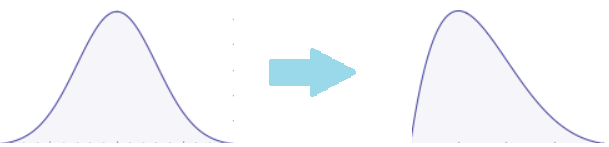
\includegraphics[width=0.7\textwidth]{images/emd.png}
\caption{Vizualizacija ideje udaljenosti pomicanja zemlje}
\label{emd}
\end{figure}

Problem u izrazu \ref{em_distance} jest što je vremenski veoma skupo odrediti traženi infinum skupa. Autori se zato koriste Kantorovič -- Rubinsteinovom dualnosti gdje se Wassersteinova udaljenost reformulira na sljedeći način:
\begin{equation}
\label{kr_dual}
W(P, Q) = \sup_{\|f\|_L \leq 1} \mathbb{E}_{x \sim P} \left[f(x)\right] - \mathbb{E}_{x \sim Q}\left[f(x)\right]
\end{equation}
Ovdje $\sup$ označava supremum skupa - najmanju vrijednost veću od svih elemenata skupa. U ovom slučaju, tražimo supremum po svim funkcijama $f : \mathcal{X} \rightarrow \mathbb{R}$ koje zadovoljavaju 1-Lipschitzovu neprekidnost. Ovo je nešto stroži zahtjev od same neprekidnosti. Općenito, $K$-Lipschitzova neprekidnost \citep{lip_cont} funkcije znači da, odaberemo li bilo koje dvije točke na grafu, apsolutna vrijednost nagiba njihove spojnice bit će manja od $K$. Vizualno, možemo provjeriti je li to svojstvo zadovoljeno u nekoj točki funkcije ako povučemo pravce nagiba $K$ kroz danu točku (slika \ref{lip_cont}).
 
\begin{figure}[h]
\centering
		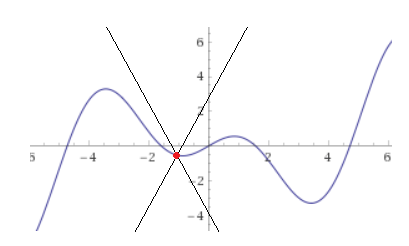
\includegraphics[width=0.7\textwidth]{images/lip_cont.png}
\caption{Vizualno ispitivanje $K$-Lipschitzove neprekidnosti. Ako kroz danu točku povučemo pravce čija je apsolutna vrijednost nagiba $K$, ravninu dijelimo na 4 dijela. Ako se ostatak grafa tada ne nalazi u gornjem i donjem području ravnine opisanom pravcima, tada je uvjet neprekidnosti zadovoljen.}
\label{lip_cont}
\end{figure}

Nadalje, može se pokazati da, ako u izrazu \ref{kr_dual} odaberemo $K > 1$, rezultat će biti $K \cdot W(P, Q)$. Ako imamo klasu funkcija parametriziranu parametrima $\vec{\theta}$ (ovo je u našem slučaju diskriminator), gdje sve zadovoljavaju Lipschitzovu neprekidnost za neki $K$, i optimum se postiže za neke $\vec{\theta}^*$, dobivamo vrijednost $K \cdot W(P, Q)$. Dakle, izraz \ref{kr_dual}, u kontekstu generativnih suparničkih mreža, možemo formulirati u sljedeći optimizacijski problem:
\begin{equation}
\max \mathbb{E}_{\vec{x} \sim p_{\mathcal{D}}} \left[D(\vec{x})\right] - \mathbb{E}_{\vec{z} \sim p_{\vec{z}}}\left[D(G(\vec{z}))\right]
\end{equation}
Iz ovog izraza, lako je odrediti gradijent generatora i diskriminatora koji su nam potrebni da bismo ih istrenirali. Jedini zahtjev je da diskriminator zadovoljava 1-Lipschitzovu neprekidnost. U tu svrhu, autori predlažu ograničavanje težina na neki mali interval, npr. [-0.1, 0.1]. Iako su postigli zadovoljavajuće rezultate, napominju da je pristup vrlo jednostavan i ostavlja prostor za druge metode osiguravanja traženog ograničenja.

Koja bi bila prednost ove funkcije gubitka u odnosu na originalno predloženu? Autori su pokazali da obje ranije predložene varijante imaju problem s iščezavajućim gradijentima, dok njihova funkcija gubitka rezultira konzistentnim gradijentima tijekom treniranja. Još jedna važna razlika u odnosu na originalan gubitak jest da izlaz diskriminatora u ovom slučaju nije vjerojatnost te zato nije ni ograničen.

\subsection{Gubitak najmanjih kvadrata}
Gubitak najmanjih kvadrata \citep{mao2016squares} razvijen je s istom motivacijom kao i Wassersteinov gubitak: da bi se izbjegao problem iščezavajućih gradijenata. Budući da originalna formulacija funkcije gubitka koristi sigmoidalnu funkciju pri klasifikaciji, gradijent za uzorke koji uspješno zavaraju diskriminator (tj. koji se nalaze s dobre strane decizijske granice), a koji su još uvijek prilično različiti od stvarnih primjera, jest nizak (slika \ref{ls_sigm}). 

\begin{figure}[h]
\centering
		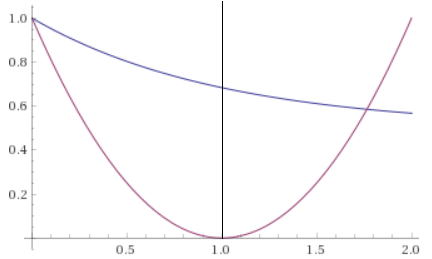
\includegraphics[width=0.7\textwidth]{images/ls_sigm.png}
\caption{Vizualna usporedba gubitka sigmoide (plavo) i kvadratnog gubitka (ljubičasto). Crno je naznačena granica između ispravno i neispravno klasificiranih primjera.}
\label{ls_sigm}
\end{figure}

Zato autori predlažu pogrešku najmanjih kvadrata za funkciju gubitka. Recimo da smo stvarne primjere označili s $a$, lažne s $b$, dok smo s $c$ označili vrijednost kojoj generator teži da bude izlaz diskriminatora. Tada bi optimizacijski problemi za generator $G$ i diskriminator $D$ glasili:
\begin{equation}
\label{ls_d}
\min_D V(D) = \frac{1}{2}\mathbb{E}_{\vec{x} \sim p_{\mathcal{D}}}\left[(D(\vec{x}) - b)^2\right] + \frac{1}{2}\mathbb{E}_{\vec{z} \sim p_{\vec{z}}}\left[(D(G(\vec{z})) - a)^2\right]
\end{equation}
\begin{equation}
\label{ls_g}
\min_G V(G) = \frac{1}{2}\mathbb{E}_{\vec{x} \sim p_{\mathcal{D}}}\left[(D(\vec{x}) - c)^2\right] + \frac{1}{2}\mathbb{E}_{\vec{z} \sim p_{\vec{z}}}\left[(D(G(\vec{z})) - c)^2\right]
\end{equation}
Radi simetričnosti, uključili smo izraz koji koristi samo izlaz diskriminatora u izraz \ref{ls_g}. Pri optimizaciji ova matematička akrobacija ne utječe na rezultat jer se spomenuti izraz gubi prilikom računanja gradijenta, ali olakšava dokazati određene povoljne karakteristike ovog gubitka. Naime, pomoću izraza \ref{ls_d} i \ref{ls_g} možemo pokazati da minimizacija gubitka najmanjih kvadrata vodi prema minimizaciji Pearsonove $\chi^2$ divergencije, još jedne mjere za udaljenost između dvije distribucije. Pearsonova $\chi^2$ divergencija između distribucija $P$ i $Q$ definirana je kao $D_{\chi^2}(P\|Q) = \int_{\mathcal{X}} (\frac{(P(x) - Q(x))^2}{Q(x)}dx$

Iz izraza \ref{ls_d} možemo pronaći optimalni diskriminator $D^*$ ako fiksiramo generator $G$. Uz fiksirani generator, \ref{ls_g} postaje
\begin{align}
V(D) &= \frac{1}{2}\mathbb{E}_{\vec{x} \sim p_{\mathcal{D}}}\left[(D(\vec{x}) - b)^2\right] + \frac{1}{2}\mathbb{E}_{\vec{x} \sim p_{model}}\left[(D(\vec{x}) - a)^2\right] \\
	&= \frac{1}{2} \int_{\mathcal{X}} \left[ p_{\mathcal{D}}(\vec{x})(D(\vec{x}) - b)^2 + p_{model}(\vec{x})(D(\vec{x}) - a)^2\right]dx
\end{align}
Podintegralna funkcija je oblika $F(y) = \frac{1}{2} \left[ e(y - b)^2 + f(y - a)^2\right]$. Lako je pokazati da je minimum ove funkcije u točki $y^* = \frac{b\cdot e + a \cdot f}{e + f}$. Obavimo li potrebne supstitucije, dobivamo:
\begin{equation}
D^*(\vec{x}) = \frac{bp_{\mathcal{D}}(\vec{x}) + ap_{model}(\vec{x})}{p_{\mathcal{D}}(\vec{x}) + p_{model}(\vec{x})}
\end{equation}
Uvrstimo li dobiveni izraz u \ref{ls_g}, dobivamo:
\begin{align*}
2V(G) &= \mathbb{E}_{\vec{x} \sim p_{\mathcal{D}}}\left[(D^*(\vec{x}) - c)^2\right] + \mathbb{E}_{\vec{x} \sim p_{model}}\left[(D^*(\vec{x}) - c)^2\right] \\
	&= \int_{\mathcal{X}} \left(p_{\mathcal{D}}(\vec{x}) + p_{model}(\vec{x})\right)\left(D^*(\vec{x}) - c\right)^2dx \\
	&= \int_{\mathcal{X}} \left(p_{\mathcal{D}}(\vec{x}) + p_{model}(\vec{x})\right) \left(\frac{(b - c)p_{\mathcal{D}}(\vec{x}) + (a - c)p_{model}(\vec{x})}{p_{\mathcal{D}}(\vec{x}) + p_{model}(\vec{x})}\right)^2 dx
\end{align*}
Radi jednostavnosti, postavimo $b - c = 1$ i $a - c = -1$. Tada imamo:
\begin{align*}
2V(G) &= \int_{\mathcal{X}} \frac{\left(p_{\mathcal{D}}(\vec{x}) - p_{model}(\vec{x})\right)^2}{p_{\mathcal{D}}(\vec{x}) + p_{model}(\vec{x})} dx
	&= \int_{\mathcal{X}} \frac{\left(p_{\mathcal{D}}(\vec{x}) + p_{model}(\vec{x}) - 2p_{model}(\vec{x})\right)^2}{p_{\mathcal{D}}(\vec{x}) + p_{model}(\vec{x})} dx \\
	&= D_{\chi^2}(2p_{model}\|p_{model} + p_{\mathcal{D}})
\end{align*}
Ovime smo dokazali da pronalazak optimalnih težina pomoću ovog gubitka minimizira Pearsonovu $\chi^2$ divergenciju između $2p_{model}$ i $p_{model} + p_{\mathcal{D}}$. Kako je ona nenegativna, postiže minimum upravo u $p_{model} = p_{\mathcal{D}}$.

Da bi ovaj rezultat vrijedio, potrebno je osigurati da vrijedi $b - c = 1$ i $a - c = -1$. Najjednostavnije rješenje je postaviti $a = -1, b = 1$ i $c = 0$. Međutim, u praksi se pokazalo da nema prevelike razlike u rezultatima ni ako postavimo $b = c = 1$ i $a = 0$, kako uobičajeno označavamo pozitivne i negativne primjere kod klasifikacije. Tako autori u svom radu koriste 
\begin{equation*}
\min_D V(D) = \frac{1}{2}\mathbb{E}_{\vec{x} \sim p_{\mathcal{D}}}\left[(D(\vec{x}) - 1)^2\right] + \frac{1}{2}\mathbb{E}_{\vec{z} \sim p_{\vec{z}}}\left[(D(G(\vec{z})))^2\right],
\end{equation*}
\begin{equation*}
\min_G V(G) = \frac{1}{2}\mathbb{E}_{\vec{z} \sim p_{\vec{z}}}\left[(D(G(\vec{z})) - 1)^2\right].
\end{equation*}


Dosad smo u ovom radu predstavili tri funkcije gubitka koje se najčešće koriste: varijantu originalne funkcije gubitka koja izbjegava zasićenje pri početku učenja, Wassersteinovu funkciju gubitka i gubitak najmanjih kvadrata. Pokazali smo i da minimiziraju odgovarajuće divergencije i da su u sva tri slučaja asimptotski konzistentni. Prirodno se postavlja pitanje: koja je od njih najbolja? Recimo ukratko da ne postoji jedinstven odgovor, jer on ovisi i o odabiru ostalih komponenti generativnih suparničkih mreža \citep{lucic2017gans}. Više riječi o odabiru komponenti kod treniranja generativnih suparničkih mreža bit će u odjeljku \ref{prijasnji_rad}. 
\section{Normalizacijske i regularizacijske tehnike}
Prenaučenost je jedna od najvećih izazova pri treniranju modela strojnog učenja, a opisuje situaciju u kojoj pokušava naučiti ne samo važne trendove u podatcima, nego i šum koji neizbježno s njima dolazi. Osnovni načini kojima pokušavamo minimizirati vjerojatnost ovog problema jest korištenjem regularizacije i normalizacije. Regularizacija je bilo koja tehnika kojom, djelovanjem na parametre modela, težimo poboljšati sposobnost generalizacije, dok kod normalizacije utječemo na ulaze modela (kod neuronskih mreža, svakog sloja zasebno). S napretkom u istraživanju dubokih mreža, napredovale su i tehnike regularizacije i normalizacije. U ovom odjeljku, ukratko ćemo predstaviti metode koje se često koriste pri treniranju generativnih suparničkih modela.

\todo{spectral norm, l2 reg, gp pen, batchnorm, layernorm}
\subsection{Regularizacija}
\subsubsection{$L_2$ regularizacija}
$L_2$ regularizacija oblik je regularizacije koji je vrlo raširen ne samo u treniranju dubokih mreža, nego i kod ostalih modela strojnog učenja. Osnovna pretpostavka jest da modeli koji postaju prenaučeni, postaju vrlo osjetljivi na male varijacije u ulaznim podatcima. Ovo se manifestira kao parametri koji imaju veliku normu te tako pojačavaju efekt šuma. Ideja je da na neki način ograničimo njihovu normu, što možemo postići malom modifikacijom funkcije gubitka modela. Pretpostavimo da model ima funkciju gubitka $L(\vec{x};\vec{\theta})$. Tada bi model s $L_2$ regularizacijom imao sljedeću funkciju kao funkciju gubitka:
\begin{equation*}
L^*(\vec{x};\vec{\theta}) = L(\vec{x};\vec{\theta}) + \frac{\lambda}{2}\|\vec{\theta}\|_2^2, 
\end{equation*}
gdje je $\|\vec{\theta}\|_2$ $L_2$ norma parametara modela. Ovime kažnjavamo model s prevelikim parametrima, a hiperparametar $\lambda$ određuje kompromis između minimizacije funkcije gubitka i norme parametara. 

Osim $L_2$ norme, u praksi se koriste i $L_1$ te $L_0$ da bi se ograničili parametri. Međutim, u kontekstu generativnih suparničkih mreža, najpovoljnija je upravo $L_2$ norma jer je svuda derivabilna, što nije istinito za ostale ovdje navedene norme.

\subsubsection{Spektralna normalizacija}
Spektralna normalizacija \todo{ref spektralna normalizacija paper} zapravo je vrsta regularizacije jer utječe na težine modela, unatoč svome imenu, i karakteristično se koristi samo kod generativnih suparničkih modela. Ideja ove tehnike leži u činjenici da se povoljnim za stabilnost treniranja pokazala $K$-Lipschitzova neprekidnost diskriminatora. \todo{mozda ref Guo-Jun Qi. Loss-sensitive generative adversarial networks on lipschitz densities ??? tamo bi to moglo pisat} Prema definiciji, Lipschitzova norma vektorske funkcije $g(\vec{x})$ jest $\|g\|_{Lip} = \sup_{\vec{x}}\sigma(\nabla g(\vec{x}))$, gdje je $\sigma(A)$ spektralna norma matrice $A$, tj. 
\begin{equation}
\sigma(A) = \|A\|_2 = \sqrt{\lambda(A^T A)},
\end{equation}
a $\lambda$ je najveća svojstvena vrijednost matrice matrice $A^T A$. Za linearni sloj duboke mreže s matricom težina $W$, dobivamo $\|g\|_{Lip} = \sup_{\vec{x}}\sigma(\nabla g(\vec{x})) = \sup_{\vec{x}}\sigma(W) = \sigma(W)$. Koristeći činjenicu da je $\sigma(p \cdot W) = p \cdot \sigma(W)$, što je trivijalno za pokazati, vrijedi da je $\sigma(W / \sigma(W)) = 1$, odnosno promatrani linearni sloj zadovoljava 1-Lipschitzovu neprekidnost. Nadalje, iz svojstva $\|g_1 \circ g_2\|_{Lip} \leq \|g_1\|_{Lip} \cdot \|g_2\|_{Lip}$, slijedi i da je cijela mreža 1-Lipschitz neprekidna funkcija ako to svojstvo vrijedi za svaki sloj. Zato regulariziramo težine sloja $k$ kao $W_k \leftarrow  W_k / \sigma(W_k)$.
Međutim, u praksi je preskupo u svakom koraku optimizacije izračunavati svojstvene vrijednosti. Autori zato predlažu brzu metodu aproksimacije koju izlažu u svom radu, ali ona izlazi izvan opsega ovoga rada.

\subsubsection{Gradijentna kazna}
Gradijentna kazna \engl{Gradient penalty} \todo{ref gradient penalty paper} također je tehnika kojim se pokušava osigurati Lipschitzova neprekidnost diskriminatora. Analizirajući učenje diskriminatora kad se koristi Wassersteinov gubitak uz ograničavanje težina na interval $[-c, c]$, autori su primijetili da 1) diskriminator nije sposoban modelirati složene funkcije te 2) ovisno o odabiru konstante $c$, učenje može rezultirati iščezavajućim ili eksplodirajućim gradijentima. Predložena alternativa temelji se na činjenici da optimalni diskriminator ima gradijent norme jednak 1, koju su autori dokazali u spomenutom radu. Zato predlažu sljedeću modifikaciju funkcije gubitka diskriminatora:
\begin{equation}
L^* = \mathbb{E}_{\vec{z} \sim p_{\vec{z}}}\left[D(G(\vec{z}))\right] - \mathbb{E}_{\vec{x} \sim p_{\mathcal{D}}} \left[D(\vec{x})\right] + \lambda \mathbb{E}_{\vec{\hat{x}} \sim p_{\vec{\hat{x}}}} \left[\left(\|\nabla_{\vec{\hat{x}}} D(\vec{\hat{x}})\|_2 - 1 \right) ^2 \right] 
\end{equation}
U odnosu na originalni optimizacijski problem, formulirali smo zadatak kao minimizaciju umjesto maksimizacije. Dodatni član u izrazu služi da bi se kaznio gradijent koji previše odstupa od optimalne vrijednosti, a $\lambda$ je hiperparametar kojim modeliramo jakost kazne (autori predlažu $\lambda = 10$. Osim toga, pokazuje se da je skupo kažnjavati gradijent svuda: autori predlažu odabir nasumične točke na spojnici uzoraka iz $p_{\mathcal{D}}$ i $p_{model}$ prema uniformnoj distribuciji te kažnjavanje gradijenta u toj točki. \todo{vizualiziraj to}

Potrebno je napomenuti i da je ovaj oblik regularizacije vremenski nešto složeniji od prethodno navedenih, ali nije ograničen samo na Wassersteinov gubitak, nego se vrlo lako mogu ugraditi i druge funkcije gubitka.

\subsection{Normalizacija}
\subsubsection{Normalizacija nad grupom}
Normalizacija nad grupom \engl{Batch Normalization} \todo{ref rad} temelji se na opažanju da je treniranje mreža lakše ako su im na ulazu normalizirani podatci. Kako se mreža sastoji od više slojeva, cilj bi nam bio da svaki sloj primi normalizirani ulaz, uz razuman vremenski trošak. Budući da mrežu učimo na manjim grupama podataka, možemo procijeniti očekivanje $\vec{\mu}$ i varijancu $\sigma^2$ svake grupe te pomoću njih normalizirati grupu:
\begin{equation}
\hat{\vec{x}} = \frac{\vec{x} - \vec{\mu}}{\sqrt{\vec{\sigma}^2 + \epsilon}}
\end{equation}
Operacija korjenovanja, kvadriranje i dijeljenje u ovom se slučaju odvijaju po elementima, a $\epsilon$ jest mala konstanta dodana u izraz radi numeričke stabilnosti. Iako nam je potrebna minigrupa da bismo odredili očekivanje i varijancu, dimenzionalnost tih vektora ovisi o dimenzionalnosti vektora $\vec{x}$, a ne broju uzoraka u minigupi. Kako ipak tijekom normalizacije gubimo određenu sposobnost reprezentacije zbog gubitka srednje vrijednosti i odstupanja, nakon normalizacije afino transformiramo dobiveni vektor:
\begin{equation}
\label{affine}
\vec{h} = \vec{\alpha}^T\vec{\hat{x}} + \vec{\beta}
\end{equation}
$\vec{\alpha}$ i $\vec{\beta}$ tada također postaju parametri koje učimo gradijentnim spustom, ali nam omogućavaju lakšu manipulaciju distribucijom izlaza svakog sloja - uobičajeno je da se normalizacija nad grupom primjenjuje prije aktivacijske funkcije. 

Još jedno važno implementacijsko pitanje je kako koristiti normalizaciju nad grupom nakon što je model naučen. Naime, nakon što se učenje završi, više se podatci ne predaju modelu u minigrupama, nego mora biti omogućeno i obrada pojedinačnih ulaza. Zato se u fazi eksploatacije koriste druge vrijednosti za očekivanje i varijancu, dobivene temeljem očekivanja i varijanci svih minigrupa tijekom učenja:
\begin{equation}
\vec{\mu} = \mathbb{E}\left[\mu_k\right], \quad \vec{\sigma}^2 = \mathbb{E}\left[\vec{\sigma}^2_k\right]
\end{equation}

\subsubsection{Normalizacija sloja}
Normalizacija sloja \todo{ref Layer Normalization} metoda je normalizacije razvijena zbog neprikladnosti normalizacije po grupama za mreže s povratnim vezama, a u kontekstu generativnih suparničke mreža prvi put je primijenjena nešto kasnije \ref{Improved Training of Wasserstein GANs} iz sličnog razloga. Naime, koristimo li normalizaciju po grupama, učimo diskriminator mapiranju između \textit{minigrupe ulaza u minigrupu izlaza}, što potencijalno uvodi korelaciju među primjerima. S druge strane, gradijentnom kaznom kažnjavamo gradijent diskriminatora za svaki primjer zasebno što zahtijeva metodu normalizacije koja ne uvodi korelaciju među ulazima. Ovdje na scenu stupa normalizacija po sloju. Ideja je da se očekivanje i varijanca odrede prema izlazima sloja za jedan primjer, umjesto prema minigrupi. Ako pretpostavimo da redovi matrice $H$ sadrže izlaze nekog sloja za danu minigrupu: u slučaju normalizacije po minigrupama, potrebne parametre procjenjujemo po redovima matrice $H$, a u slučaju normalizacije po sloju, po stupcima dane matrice. Tako izlaz za svaki primjer kod normalizacije sloja ima vlastito očekivanje i varijancu. Odredivši parametre, normaliziramo izlaz prema
\begin{equation}
\hat{\vec{x}} = \frac{\vec{x} - \vec{\mu}}{\sqrt{\vec{\sigma}^2 + \epsilon}}
\end{equation}
te primjenjujemo afinu transformaciju na dobiveni vektor (izraz \ref{affine}). Kao i ranije, učimo parametre afine transformacije.

Prednosti ovog pristupa su što ne postoji razlika u korištenju sloja tijekom faze eksploatacije u odnosu na fazu korištenja, primjenjiva je i kad veličina minigrupe nedovoljna za dobru aproksimaciju očekivanja i varijance, osigurava da su izlazi sloja za različite primjere međusobno neovisni, ali uvode korelaciju između izlaza za isti primjer.
\section{Arhitektura dubokih mreža}
Duboke neuronske mreže pronašle su svoju primjenu u rješavanju mnogih zadataka strojnog učenja kao što su klasifikacija slika, analiza teksta, predviđanje vremenskih serija i sl. Pokazalo se nužnim, međutim, razviti nove slojeve neuronskih mreža da bi se ugradile pretpostavke prilagođene trenutnom zadatku. U ovom odjeljku predstavit ćemo slojeve koji se uobičajeno koriste u generatoru i diskriminatoru generativnih suparničkih mreža te aktivacijske funkcije primijenjene na njihove izlaze.

\subsection{Potpuno povezani sloj}
Potpuno povezani sloj je najjednostavniji sloj u neuronskoj mreži, a predstavlja afinu transformaciju ulaza u izlaz, tj. izlaz svakog neurona predstavlja linearnu kombinaciju ulaza kojoj je pribrojen neki konstantni faktor. Matrično, ovo možemo zapisati kao:
\begin{equation}
\vec{h} = W\vec{x} + \vec{b}
\end{equation}
gdje je $W$ matrica težina za svaki neuron, a $\vec{b}$ vektor pomaka koje pribraja. Tako je dimenzionalnost matrice $W$ $H \times N$, gdje je $N$ broj elemenata vektora na ulazu, a $H$ broj neurona u sloju. Naravno, $\vec{b}$ je $H$-elementni vektor jer je izlaz operacije $W\vec{x}$ istog broja elemenata.

Uobičajeno se koristi kao zadnji sloj u diskriminatoru da mapira izlaze prethodnih slojeva na skalarni izlaz, ili kao prvi sloj u generatoru da transformira ulazni slučajni vektor $\vec{z}$ u izlaz koji je uglavnom veće dimenzionalnosti. Neki autori \citep{karras2019style} u ovu svrhu koriste i više naslaganih potpuno povezanih slojeva uz manju modifikaciju o kojoj će više riječi biti kasnije.

\subsection{Konvolucijski sloj} 
Osnovna je zadaća konvolucijskoga sloja procesuiranje ulaza za koji znamo da je rešetkaste strukture \citep{Goodfellow-et-al-2016}, kao što su slike. Ime su dobile po tome što se umjesto operacije matričnog množenja, pri određivanju izlaza, koriste diskretnom konvolucijom matrice težina, čija je oznaka $*$. Dakle, određivanje izlaza konvolucijskog sloja možemo zapisati kao:
\begin{equation}
H = W * X + B
\end{equation}
Budući da su nam ulazi, u kontekstu generativnih suparničkih modela, slike, $X$ jest tenzor trećeg reda (visina, širina i broj kanala slike), kao i $H$ te $B$, dok je matrica težina $W$ tenzor četvrtoga reda (broj ulaznih kanala, broj izlaznih kanala, širina i visina prozora). $W$ u kontekstu konvolucijskoga sloja još nazivamo jezgrom, a $H$ mapom značajki. 
Izraz za diskretnu konvoluciju glasi:
\begin{equation}
(K * I)(i, j) = \sum_m\sum_nI(i - m, j - n)K(m, n)
\end{equation}
Primijetimo da je ovaj izraz prilagođen slučaju gdje su $K$ i $I$ tenzori drugoga reda. Međutim, vrlo lako možemo proširiti ovu definiciju kratkom analogijom s potpuno povezanim slojem. Kod potpuno povezanoga sloja, možemo primijetiti da težina $w_{ij}$ povezuje $i$-ti ulaz s izlazom $j$-toga neurona. U konvolucijskom sloju, tenzori su dimenzija $H_1 \times W_1 \times C_1$ i $H_2 \times W_2 \times C_2$, a već smo "osigurali" povezanost između visina $H_1, H_2$ i širina $W_1, W_2$. Ostaje nam još povezati mape značajki kojih ima $C_1$ u ulazu i $C_2$ na izlazu - u tu svrhu jednostavno alociramo konvolucijske jezgre za svako mapiranje (dakle, ima ih $C_1 \times C_2$). Formalno, $r$-ta mapa značajki određuje se kao:
\begin{equation}
H^{(r)} = \sum_s X^{(s)} * W^{(r, s)}
\end{equation}

Intuitivno, jezgre možemo zamisliti kao "prozore" određenih dimenzija kojima klizimo preko ulazne "slike" te izlazna vrijednost te operacije ovisi samo o vrijednostima koje su vidljive unutar prozora, čime konvolucija modelira efektivno modelira samo lokalne interakcije. Slika \ref{conv} vizualizira ovu ideju. Parametri prozora nisu ovisni o njegovoj poziciji, nego ostaju konstanti tijekom prijelaza. Time značajno smanjuje broj potrebnih parametara i omogućuje ekvivarijantnost na pomak. Funkcija $f$ je ekvivarijantna s obzirom na $g$ ako vrijedi $f \circ g = g \circ f$. U slučaju konvolucije, ako pomaknemo ulaz, pomaknut će se i mapa značajki, što je povoljno svojstvo kod obrade slika.

\begin{figure}[h]
\centering
		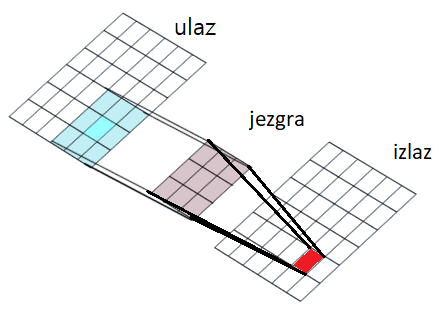
\includegraphics[width=0.8\textwidth]{images/conv.png}
\caption{Vizualizacija konvolucije.}
\label{conv}
\end{figure}

Kod uporabe konvolucijskog sloja, postoji nekoliko odluka koje korisnik mora donijeti između kojih je odabir pomaka prozora (ne mora se nužno prozor pomicati za samo jedan piksel), smanjivanje dimenzionalnosti izlaznog tenzora i broj izlaznih mapa značajki. Osvrnimo se kratko na problem smanjivanja dimenzionalnosti. Pretpostavimo da je ulazna slika dimenzija $H \times W$ (mape značajki u ovom trenutku nisu važne). Primijenimo li konvoluciju s jezgrom dimenzije $K \times K$, izlaz će biti $H - K +  1 \times W - K + 1$, a ne $H \times W$. To je ponekad poželjna funkcionalnost, ali češće bismo željeli da dimenzije slike ne opadaju s veličinom jezgre jer se konvolucijski slojevi često koriste slijedom jedan iza drugoga. Standardno je rješenje dodati $\left \lfloor \frac{k}{2} \right \rfloor$ nula sa svih strana ulaza čime izlaz postaje željenih dimenzija.

Može se pokazati da je gradijent konvolucije ponovno konvolucija, ovaj put gradijenata funkcije gubitka po izlazu sa jezgrom zrcaljenom oko središnjeg elementa. Ovu operaciju nazivamo transponiranom konvolucijom. Moguće ju je, također, koristiti u nekim slučajevima i u unaprijednom prolazu.

U kontekstu generativnih suparničkih mreža, konvolucija i transponirana konvolucija koriste se i u diskriminatoru i u generatoru. U diskriminatoru, koriste se kao osnovni dijelovi blokova kojim se smanjuje rezolucija ulaza - obavimo konvoluciju, rezultat propustimo kroz sloj sažimanja (o kojima ćemo nešto više reći kasnije) koji smanjuje dimenzionalnost izlaza konvolucije. Zatim novodobivene vrijednosti predamo kao ulaz idućem konvolucijskom sloju i to ponavljamo dok ulaz ne smanjimo do zadovoljavajuće veličine. 

S druge strane, u generatoru ponekad koristimo transponiranu konvoluciju s korakom većim od 1 - ovo efektivno omogućuje povećanje rezolucije slike s kojom radimo. Naime, uobičajeni pristup je generirati na početku tenzor male rezolucije (npr. $2 \times 2$) te transponiranom konvolucijom udvostručiti rezoluciju (tako da je jedan korak 2 piksela), gdje se nadamo da ćemo time popuniti nastale "rupe" dobivene širenjem tenzora nekom smislenom vrijednosti. 

Spomenimo još da, ako koristimo konvolucijski sloj gdje je korak samo 1 element, nije bitno jesmo li odabrali transponiranu ili "običnu" konvoluciju - jezgre će biti samo zrcaljene varijante jedna druge. 

\pagebreak
\subsection{Slojevi sažimanja i proširivanja}
Funkcija slojeva sažimanja i naduzorkovanja jest mijenjanje rezolucije ulaznog tenzora. Sloj sažimanja često se koristi u tandemu s konvolucijom u diskriminatoru da bi se povećalo receptivno polje značajki dubljeg sloja. Receptivno polje jest skup svih elemenata ulaznog sloja koje mogu utjecati na vrijednost te značajku. Pojasnimo na jednostavnom primjeru zašto je povećanje receptivnog polja povoljno za klasifikaciju u konvolucijskim modelima.

Pretpostavimo da naša ulazna slika prikazuje ljudsko lice. Prva konvolucija detektirala bi detalje niže razine, kao što je jedno oko, nos ili uho. Nakon što izlaz propustimo kroz sloj sažimanja, idućoj konvoluciji omogućavamo pogled na veći dio slike: tako možda uspije detektirati da ljudsko lice ima dva oka, dva uha i jedan nos. Apstrahiramo li ovaj primjer, možemo reći da sloj sažimanja omogućuje dubljim konvolucijskim slojevima modelirati značajke više razine.

Sažimanje se obično provodi određivanjem statističkih pokazatelja ulazne slike unutar nekog prozora, primjerice maksimalne ili prosječne vrijednosti. Problem smanjivanja širine i visine ulaznog tenzora koji se pojavljuje kod konvolucije prisutan je i kod sažimanja te je potrebno donijeti odluku hoćemo li nadopunjavati \engl{padding} ulaz nulama ili ne.

S druge strane, slojevi proširivanja u generatoru služe kao alternativa transponiranoj konvoluciji za povećavanje rezolucije. Naime, uporaba transponirane konvolucije često rezultira tvorevinama koje podsjećaju na šahovnicu (slika \ref{checkerboard}) \citep{odena2016deconvolution}. 

\begin{figure}[h]
\centering
		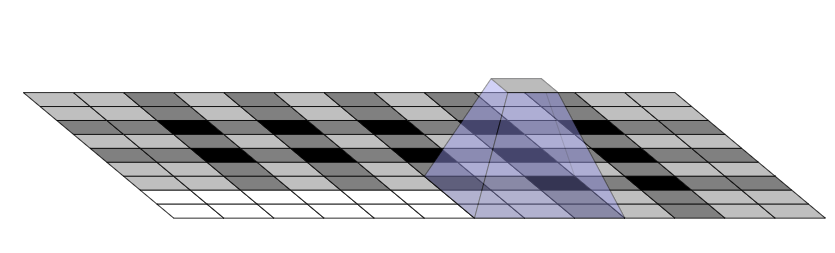
\includegraphics[width=0.8\textwidth]{images/checkers_reason.png}
\caption{Vizualizacija uzroka šahovskog uzorka. Konvoluciju s jezgrom $3 \times 3$ provodimo uz korak duljine 2. Što je element tamniji, više je elemenata uključeno u njegov izračun. Preuzeto iz \cite{odena2016deconvolution}}
\label{checkers_reason}
\end{figure}
		
\begin{figure}[h]
\centering
		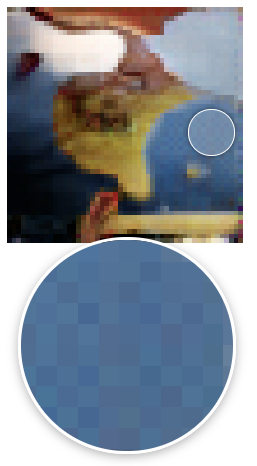
\includegraphics[height=0.5\textwidth]{images/checkers.png}
\caption{Primjer tvorevina koje podsjećaju na šahovnicu. \cite{dumoulin2016adversarially}, preuzeto s https://distill.pub/2016/deconv-checkerboard/}
\label{checkerboard}
\end{figure}

Uzrok ovome je što u nekim slučajevima određenim elementima tenzoru više rezolucije pridonosi više elemenata niže rezolucije nego ostalima (slika \ref{checkers_reason}). 

Da bi se izbjegla ova pojava, istraživači su se okrenuli kombinaciji proširivanja ulaznog tenzora i konvoluciji s jediničnim korakom (i nadopunjavanjem). Postoji nekoliko načina proširivanja, ali najčešće se, zbog jednostavnosti, koristi proširivanje uz interpolaciju pomoću najbližeg susjeda: vrijednost nepoznatih piksela povećane slike određuje se kao vrijednost najbližeg poznatog piksela. Na rezultirajući tenzor zatim primijenimo konvoluciju da bismo prilagodili vrijednosti novih piksela na finiju rezoluciju.  
\section{Dosadašnji napredak}
\label{prijasnji_rad}
U ovom odjeljku, cilj nam je predstaviti radove koji su snažno utjecali na smjer istraživanja generativnih suparničkih mreža. Iako je ovaj radni okvir definiran tek 2014. \citep{orig_paper}, atraktivno je područje u dubokom učenju te je koncept korišten u mnogim izazovima.

Spomenuli smo ranije da se istraživanje generativnih suparničkih mreža ugrubo može podijeliti u dvije grane: unaprijeđivanje kvalitete generiranih slika i poboljšavanje stabilnosti treniranja. Kako su u prethodnim odjeljcima prikazane relevantne tehnike za unaprijeđivanje treniranja, ovdje će fokus biti na napretcima u kvaliteti generiranja.

Jedno od najranijih opažanja jest da generativnim suparničkim mrežama pogoduje znanje o oznakama primjera koje trebaju generirati \citep{mirza2014conditional}. Autori su uveli malu promjenu u formulaciju minimax igre - umjesto izlaza diskriminatora $D(\vec{x})$ i generatora $G(\vec{x})$ promatramo uvjetne izlaze $D(\vec{x}\|\vec{y})$ i $G(\vec{z}\|\vec{y})$, gdje je $\vec{y}$ oznaka primjera u \textit{one-hot} obliku.

Nešto kasnije, predložene su smjernice za dizajn dubokih generativnih suparničkih mreža s konvolucijskim slojevima \citep{radford2015unsupervised} koje su postali polazna točka za istraživanje u idućim godinama. Među smjernicama su, između ostaloga, uporaba normalizacije po grupama, korištenje zglobnice kao aktivacijske funkcije te eliminacija potpuno povezanih skrivenih slojeva u mrežama.

Grupa istraživača iz tvrtke NVIDIA predložili su poboljšanu proceduru učenja generativnih suparničkih mreža koja se temelji na progresivnom učenju različitih rezolucija ulaznih slika, počevši od najmanje \citep{karras2017progressive}. Ovo je varijanta poznate tehnike za treniranje neuronskih mreža pod nazivom nadzirano predtreniranje, prilagođene za generativni problem.

Isti autori su kao nadogradnju prethodnoga modela predložili arhitekturu temeljenu na odvajanju učenja stila (koji je neovisan o rasporedu elemenata na slici) i strukture kojoj ti elementi podliježu \citep{karras2019style}. Ovim su pristupom, osim što su proizveli izvrsne rezultate, omogućili i određen stupanj kontrole nad generiranim slikama, što dotad nije bio slučaj. Stil su modelirali na zanimljiv način. Umjesto da direktno koriste slučajni vektor koji im je na ulazu, prvo ga propuste kroz nekoliko potpuno povezanih slojeva da bi razdvojili učenje ulaznog prostora od učenja viših elemenata slike. Zatim dobiveni rezultat koriste kao reprezentaciju stila koji primjenjuju na svaku rezoluciju u generatoru. Njihov rezultat predstavlja trenutni vrhunac u kvaliteti generiranih slika.

Osim toga, generativne suparničke mreže primijenjene su i na problem prevođenja slike u sliku - poznat primjer je zamjena konja na slikama zebrama i obrnuto \citep{zhu2017unpaired}. Osnovna je ideja vrlo jednostavna. Pretpostavimo da imamo početnu pretpostavku o potrebnom mapiranju i njegovu inverzu. Ukoliko je savršeno mapiranje, primijenimo li prvo njega pa njegov inverz, trebali bismo dobiti početnu sliku. Upravo ovu razliku pokušava minimizirati predloženi model.

Komentirajmo još kratko tehnike stabilizacije treniranja generativnih suparničkih mreža. Grupa autora je u dva rada \citep{kurach2018largescale}, \citep{lucic2017gans} provela brojne eksperimente kojima su ispitali dosad predložene načine učenja, tehnike regularizacije i normalizacije. Ispostavlja se da odabir funkcije gubitka ovisi o skupu podataka na kojemu radimo, ali dodatak spektralne normalizacije i gradijentne kazne poboljšavaju krajnji rezultat. Zato predlažu minimizaciju Kullback-Leiblerove divergencije uz spektralnu normalizaciju kao dobru početnu točku za primjenu generativnih suparničkih mreža na nove skupove podataka. 
\chapter{Prototipna implementacija}
Radi praktične demonstracije funkcionalnosti generativnih suparničkih mreža, implementirali smo varijantu modela temeljenu na progresivnom rastu \citep{karras2017progressive}. U ovom poglavlju, predstavit ćemo detaljno korištenu arhitekturu uz pojašnjenje specifičnosti karakterističnih upravo za ovaj tip modela. Predstavit ćemo i skup podataka na kojemu smo trenirali te dobivene rezultate.

\section{Arhitektura}
Kao što smo već ranije spomenuli, osnovna ideja kod progresivnog rasta generativnih suparničkih mreža jest slijedno treniranje na inačicama ulaznog skupa podataka rastućih rezolucija. Primjerice, početni model istreniramo na skupu slika rezolucije $4 \times 4$. Nakon što postupak optimizacije konvergira, model nadogradimo i povećamo rezoluciju na $8 \times 8$ i nastavimo s treniranjem te ovakav postupak ponavljamo dok ne postignemo željenu rezoluciju.

Da bismo pojasnili na koji način je ovaj princip učenja implementiran, pogledajmo prvo osnovnu građevnu jedinicu našeg modela: blok. Naravno, blokovi za diskriminator (slika \ref{disc_blocks}) i generator (slika \ref{gen_blocks}) se ponešto razlikuju, ali im je funkcionalnost slična. 

\begin{figure}[h]
\centering
		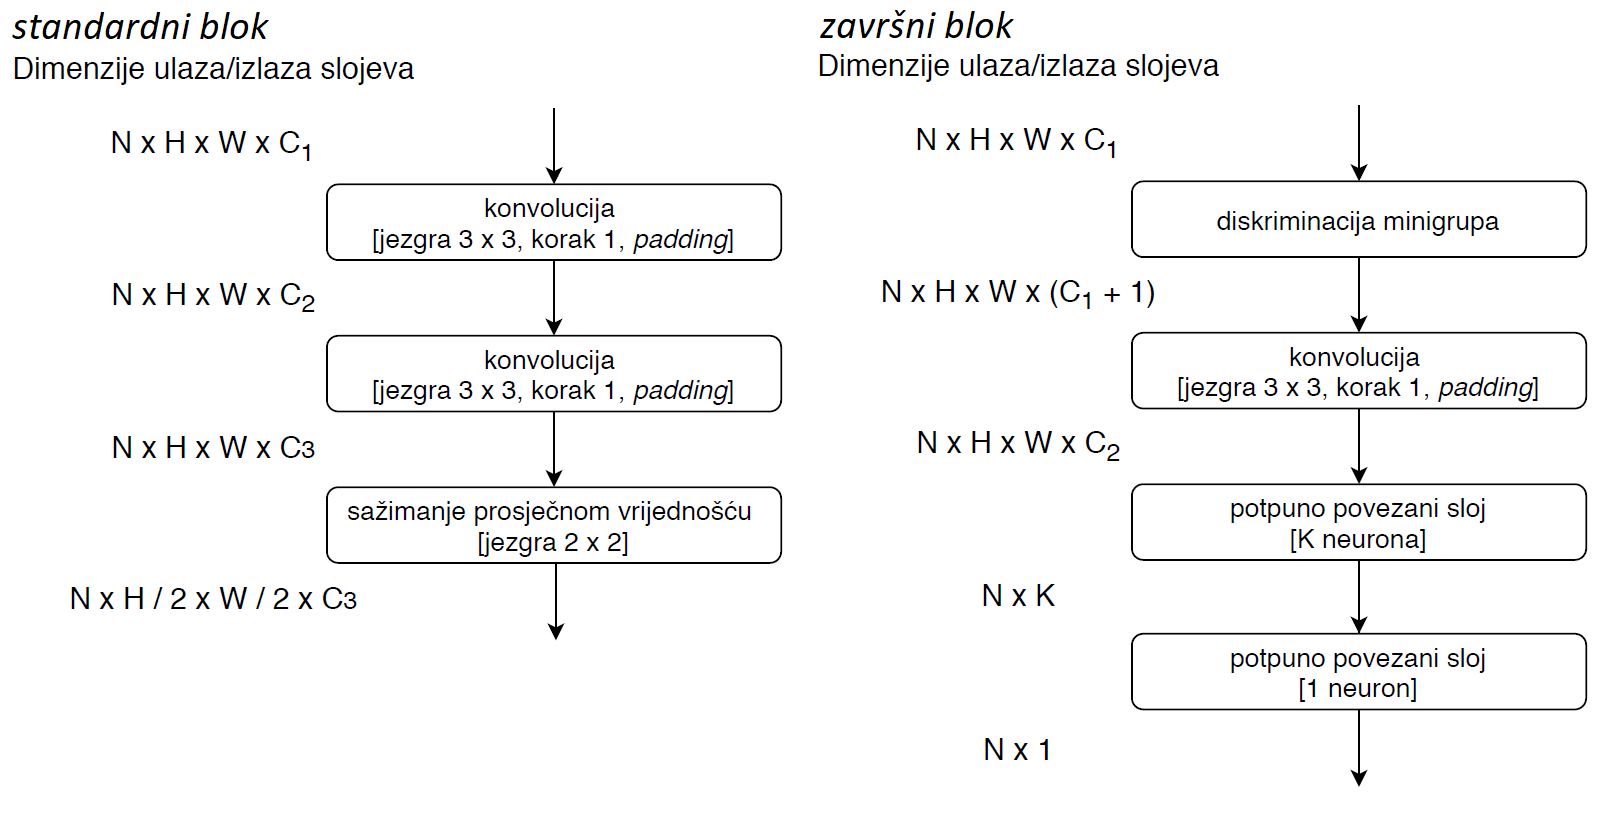
\includegraphics[height=0.5\textwidth]{images/blokovi_diskriminatora.png}
\caption{Shema korištenih blokova u diskriminatoru}
\label{disc_blocks}
\end{figure}

\begin{figure}[h]
\centering
		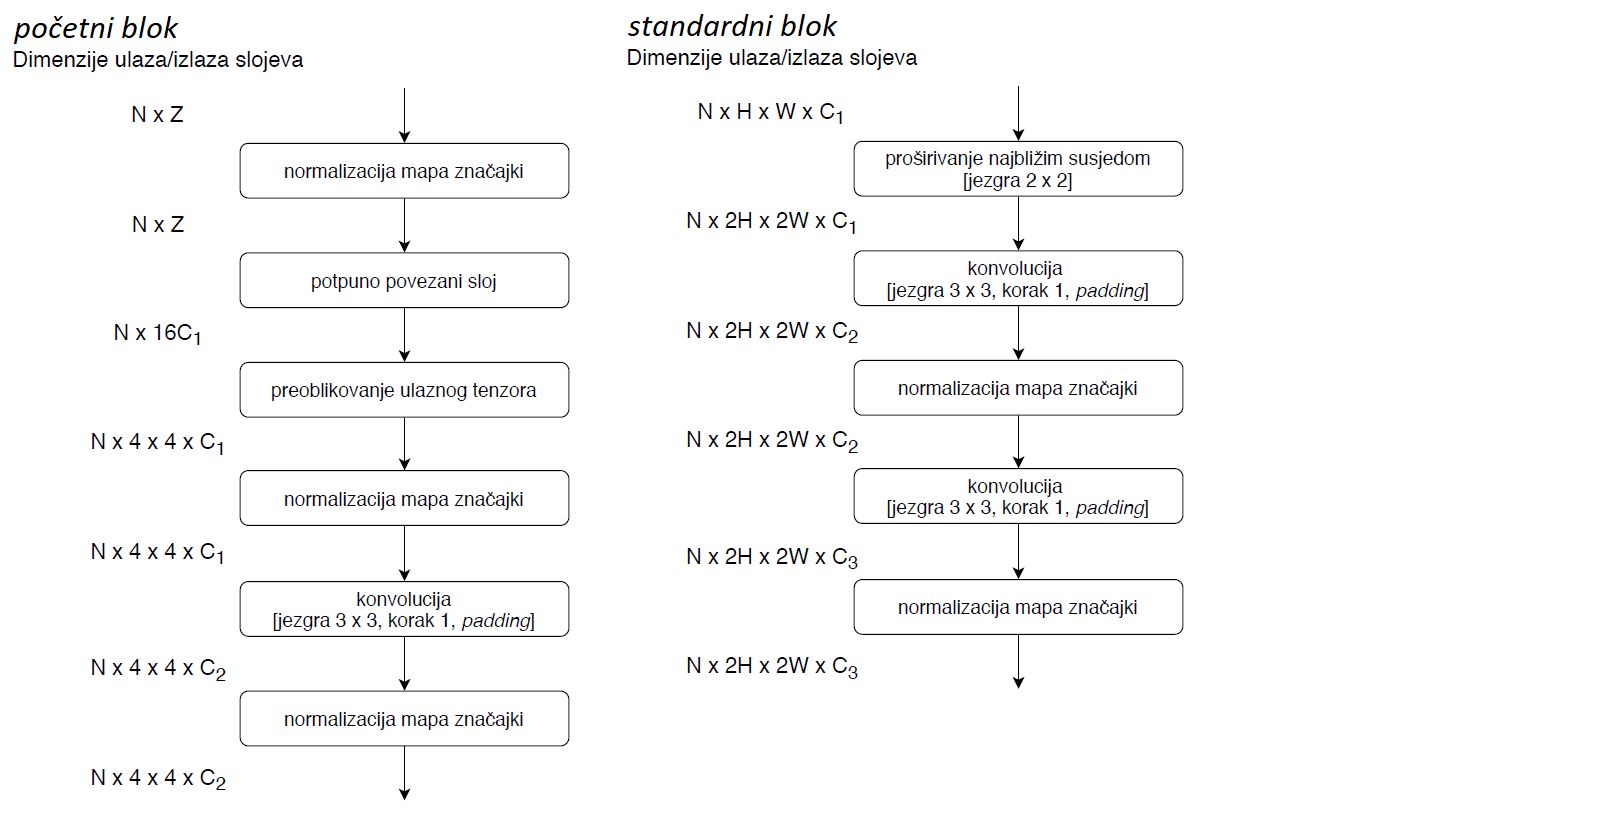
\includegraphics[height=0.7\textwidth]{images/blokovi_generatora.png}
\caption{Shema korištenih blokova u generatoru}
\label{gen_blocks}
\end{figure}

Zadaća jednog bloka jest povećati ili smanjiti rezoluciju ulaznog tenzora (ovisno radi li se o diskriminatoru ili generatoru) te ekstrahirati važne značajke dobivenog rezultata. Nadogradnja modela tada se svodi na eliminaciju izlaznog sloja te dodavanje bloka i novog izlaznog sloja na kraj (u slučaju generatora) ili eliminaciju ulaznog sloja te dodavanje bloka i novog ulaznog sloja (u slučaju diskriminatora). Ovakav pristup možemo promatrati kao tehniku nadziranog predtreniranja \citep{cupic2019nadpred} prilagođen našem zadatku. Napomenimo još da težine nižih blokova nisu "zamrznute" za vrijeme treniranja na višim rezolucijama, nego ih i dalje optimiramo pomoću gradijentnog spusta.

Osim navedenih blokova, koristimo i konvolucijske slojeve čija je zadaća osigurati tranziciju tenzora iz prostora slika (tenzora oblika $D \times D \times C$, gdje je $D$ duljina stranice slike, a $C$ broj kanala) u prostor mapa značajki, odnosno tenzora oblika $D \times D \times F$, gdje je $F$ broj mapa značajki. Razlika je što kanali predstavljaju informacije potrebne za vizualizaciju slike, dok mape značajki modeliraju i informacije o strukturi pohranjene na slikama. Ovi konvolucijski slojevi koriste se kao ulazni sloj u diskriminatoru te izlazni sloj u generatoru.

Broj mapa značajki i kod različitih rezolucija se razlikuje. Kako autori u radu ne navode kako ih određuju, za odabir broja mapa značajki koristimo prilagođenu funkciju koja se može pronaći na \citep{progressive_gan_git}.

U svim se slojevima kao aktivacijska funkcija koristi propusna zglobnica \engl{Leaky ReLU}, osim izlaznim slojevima generatora i diskriminatora gdje je aktivacijska funkcija linearna. Propusna je zglobnica definirana kao:
\begin{equation*}
f(x; \alpha) = 
	\begin{cases}
		x, \quad \text{ako } x > 0,\\
		\alpha x, \quad \text{inače} 
	\end{cases}
\end{equation*}
$\alpha$ je uobičajeno mali pozitivan broj, u našem slučaju 0.2. Popularna aktivacijska funkcija zglobnica \engl{ReLU} je specijalni slučaj propusne zglobnice gdje je $\alpha = 0$.

Da bi se smanjila vjerojatnost da se dogodi \textit{mode collapse}, \citep{salimans2016improved} predlažu postupak nazvan diskriminacijom minigrupa \engl{Minibatch Discrimination}. Osnovna ideja je proširiti neki sloj unutar diskriminatora mjerama varijacije minigrupe koji će omogućiti diskriminatoru detektirati \textit{mode collapse} te u skladu s time kazniti generator. Ovdje koristimo pojednostavljenu varijantu određivanja varijacije među elementima unutar minigrupe koja ne uvodi dodatne parametre koje moramo optimizirati.

Pretpostavimo da je naša minigrupa tenzor oblika $N \times D \times D \times F$. Za svaki element svih mapa značajki odredimo standardnu devijaciju (rezultat je tenzor oblika $D \times D \times F$). Zatim dobiveni tenzor izravnamo u jedan vektor kojemu odredimo srednju vrijednost. Dobivenom srednjom vrijednosti (samo jedan broj) popločimo dodatnu mapu značajki oblika $D \times D$ i to nadovežemo na ulaznu minigrupu, čime dobivamo izlaz $N \times D \times D \times (F + 1)$. Iako je pristup vrlo jednostavan, uspijeva poboljšati varijaciju u rezultatima koje generira naš model.

Nadalje, autori kao razlog nestabilnosti treniranja navode eksplodirajući gradijent: magnitude parametara zbog dubine modela nezaustavljivo rastu uslijed natjecanja. Problem je još izraženiji nego kod "običnih" dubokih modela jer gradijenti po parametrima ulaznog sloja generatora prolaze kroz dvostruko više slojeva što uzrokuje jaki porast magnitude u tandemu s propusnom zglobnicom koja ne ograničava pozitivne vrijednosti gradijenata. Zato uvode jako ograničenje na izlaze konvolucijskih slojeva unutar generatora: podijele izlazni tenzor na mrežu tenzora oblika $1 \times 1 \times F$ što je ekvivalentno vektoru, te svaki dobiveni vektor normaliziraju čime na efikasan način rješavaju opisani problem.

I napokon, uvedena je još jedna manja modifikacija inicijalizaciji težina. Većina arhitektura oslanjala se na pažljivu inicijalizaciju koja ovisi o broju veza koji ulaze u promatrani neuron. Razlog ovome je da bi se u izlaznom tenzoru očuvala varijanca ulaznoga. Međutim, autori inicijaliziraju parametre uzorkovanjem iz normalne distribucije $\mathcal{N}(0, 1)$ te ih dinamički skaliraju tek pri korištenju, koristeći normalizacijsku konstantu $c$ iz Heovog inicijalizatora \citep{he2015init}. Heov inicijalizator vrsta je inicijalizatora prilagođena aktivacijskoj funkciji zglobnice te osigurava da varijance ulaza i izlaza budu jednake. Dakle, nakon što smo inicijalizirali neki parametar $w$ uzorkujući normalnu distribuciju $\mathcal{N}(0, 1)$, prilikom korištenja mreže ga prilagodimo na sljedeći način:
\begin{equation*}
	\hat{w} = \frac{w}{c}, \quad c = \frac{1}{\sqrt{N}},
\end{equation*}
gdje je $N$ broj veza koje ulaze u neuron. Razlog ovakvom dinamičkom prilagođavanju težina je što moderni optimizatori (Adam, RMSProp) prilikom određivanja gradijenta ne uzimaju u obzir veličinu parametra, nego ga normaliziraju procjenom standardne devijacije. Ako neki parametar ima veći raspon od ostalih, tako će mu trebati više vremena da bude podešen što može uzrokovati da "stopa učenja bude istovremeno i prevelika i premala" \citep{karras2017progressive}. Ovakvim pristupom osiguravamo da je raspon svih parametara približno jednak.

Generator i diskriminator izvedeni su koristeći radne okvire Tensorflow \citep{tensorflow2015-whitepaper} i Keras \citep{chollet2015keras} zbog opsežne dokumentacije i objektno orijentiranog pristupa oblikovanju koji znatno olakšava oblikovanje.

\section{Učenje prototipa}

\subsection{Skup podataka za učenje}
Kao skup podataka na kojem ćemo istrenirati naš model, odabran je skup slika CelebA \citep{liu2015faceattributes}. Sastoji se od 200599 slika slavnih osoba, rezolucije $128 \times 128$. Odabran je jer pruža dovoljno dobar omjer težine zadatka (da bismo mogli pošteno demonstrirati mogućnosti generativnih suparničkih mreža) te vremenske i prostorne složenosti. 

Skup podataka pretprocesiramo pomoću modula dostupnog u repozitoriju \citep{progressive_gan_git}. Njegova je zadaća načiniti verzije originalnog skupa podataka, ali smanjene rezolucije, počevši od $4 \times 4$. Zatim se cijeli skup pohrani u binarni format .tfrecords, koji radni okvir Tensorflow vrlo efikasno može čitati s diska. Po učitavanju skupa podataka, elementi slika su transformirani s intervala $[0, 255]$  na interval $[-1, 1]$. Važno je napomenuti da spomenuti modul za pretprocesiranje slike pohranjuje u formatu $CHW$ (slika je pohranjena kao tenzor trećeg reda, element $[i, j, k]$ označava $i$-ti kanal, $j$-ti redak i $k$-ti stupac). Ovaj format prebacujemo u $HWC$ jer je to u korištenom radnom okviru pretpostavljen oblik, kao i relevantnim bibliotekama za rad sa slikama.

Skup podataka dijelimo na 2 dijela:, uzimamo prvih 200 000 slika da bismo istrenirali model, a ostatak koristimo za testiranje.

\subsection{Postupak učenja}
Koristimo algoritam Adam za učenje generatora i diskriminatora te Wassersteinov gubitak s gradijentnom kaznom kao funkciju gubitka. 

Tijekom učenja razlikujemo dvije faze: fazu stabilizacije i fazu učenja.

U fazi stabilizacije, generator i diskriminator polako se privikavaju na promjenu rezolucije da ne bismo uveli prenagle promjene u parametrima i tako poništili dotad naučeno. U generatoru, ovaj postupak izvodimo tako da, nakon što ga nadogradimo novim blokom, linearno interpoliramo između izlaza niže i više rezolucije uz parametar $\alpha$ koji ovisi o broju predočenih minigrupa (slika \ref{gen_interpolation}). 

\begin{figure}[h]
\centering
		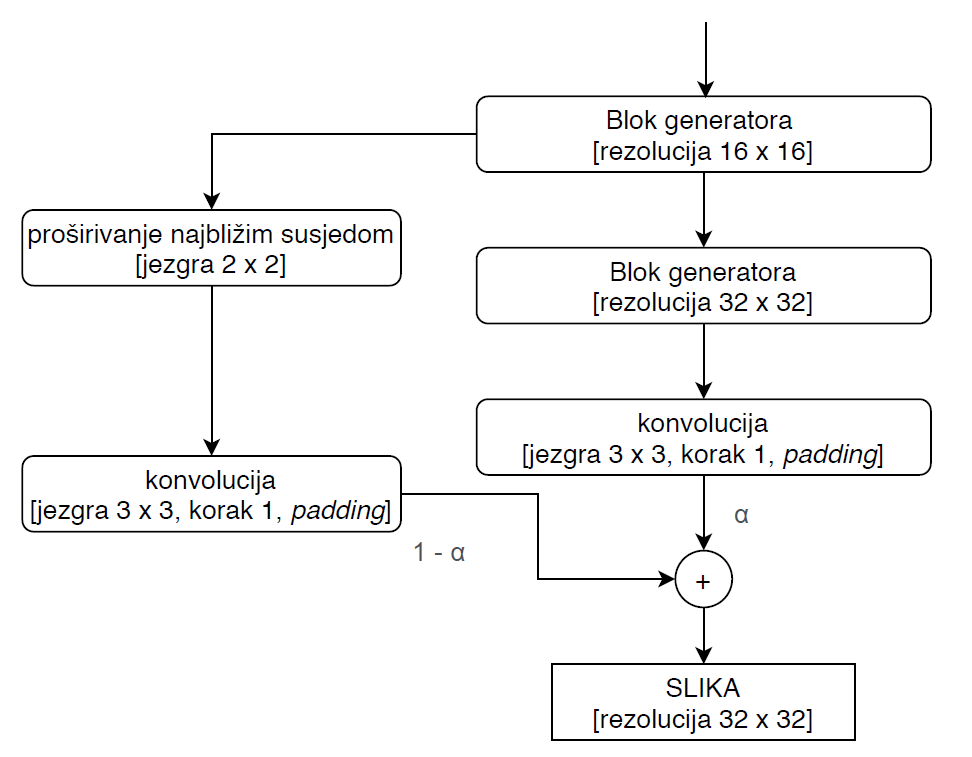
\includegraphics[height=0.7\textwidth]{images/generator_interpolation.png}
\caption{Vizualizacija interpolacije u generatoru}
\label{gen_interpolation}
\end{figure}
 
Analogno ovom postupku, odvija se i linearna interpolacija između ulaza u diskriminatoru (slika \ref{disc_interpolation}). 

\begin{figure}[h]
\centering
		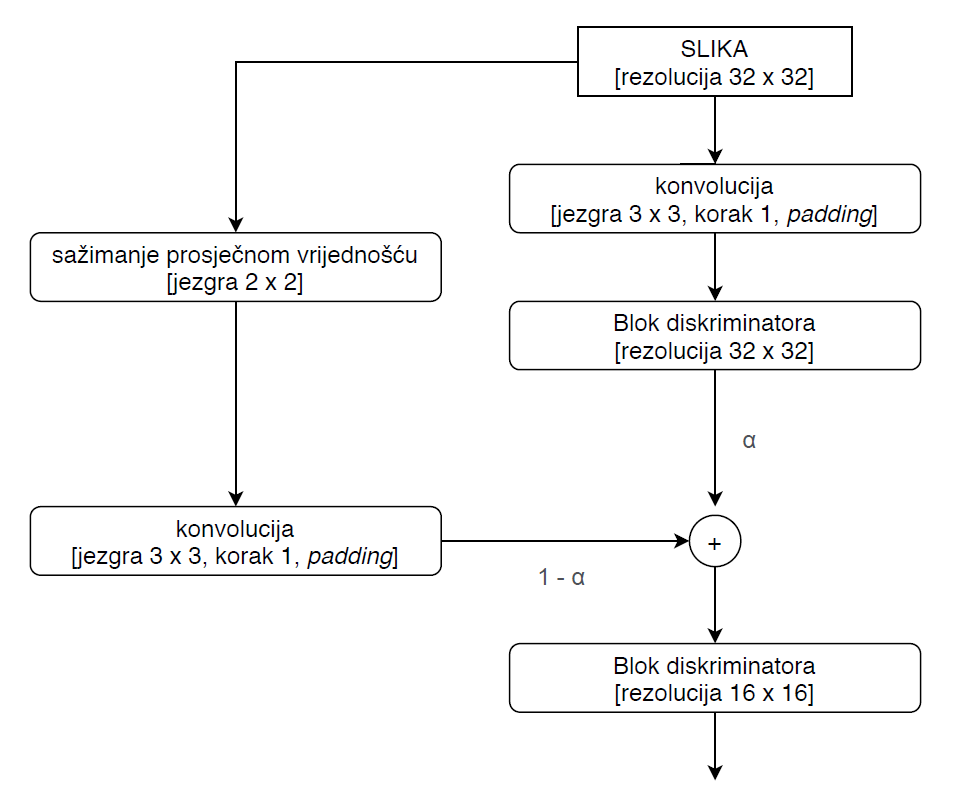
\includegraphics[height=0.7\textwidth]{images/discriminator_interpolation.png}
\caption{Vizualizacija interpolacije u diskriminatoru}
\label{disc_interpolation}
\end{figure}

Faza stabilizacije traje dok mrežama nije predočeno ukupno 800 000 stvarnih slika, odnosno 4 epohe.

Zatim nastupa faza učenja u kojoj zanemarujemo izlaz niže rezolucije, nego učimo samo pomoću više rezolucije. Kao i stabilizacija, ova faza traje dok ne predočimo 800 000 slika. Napominjemo još jednom da se uče i parametri nižih slojeva, odnosno ne zamrzavaju se.

Zbog ograničenih hardverskih mogućnosti, trenirali smo samo do rezolucije $64 \times 64$. Nakon što smo istrenirali model od najniže rezolucije do ciljne, odredili smo u kojem je trenutku treniranja model proizvodio vizualno najprihvatljivije rezultate te ponovno započeli treniranje koristeći postojeće težine kao početne, uz smanjenu stopu učenja. 

Generativna suparnička mreža istrenirana je koristeći jedan Tesla V100 GPU od 16 GB. Početna faza treniranja trajala je 30 h, od čega je 16 h na najvišoj rezoluciji te dodatnih 16 h pri rafiniranju parametara mreže. 

Korišteni hiperparametri nalaze se u tablici \ref{tablica_hiper}.

\begin{table}[h]
\caption{Korišteni hiperparametri}
\begin{center}
\begin{tabular}{|c|c|} 
 \hline
 Veličina minigrupe & 16\\ 
 \hline
 Veličina ulaznog slučajnog vektora & 512\\
 \hline
 Stopa učenja generatora & 0.001\\ 
 \hline
 Stopa učenja diskriminatora & 0.001\\ 
 \hline
 Veličina skupa za treniranje & 200000\\
 \hline
 Broj stabilizacijskih epoha & 4\\
 \hline
 Broj epoha učenja & 4\\
 \hline
 Parametar propusne zglobnice & 0.2\\
 \hline
 Parametar gradijentne kazne & 10\\
 \hline
\end{tabular}
\end{center}
\label{tablica_hiper}
\end{table}
\section{Rezultati}
Kao što smo već spomenuli, model ispitujemo na skupu slika CelebA, povećavajući rezoluciju od $4 \times 4$ do $64 \times 64$. Primjer promjene rezolucije prikazan je na slici \ref{gt_resolutions}.

\begin{figure}[h]
\centering
		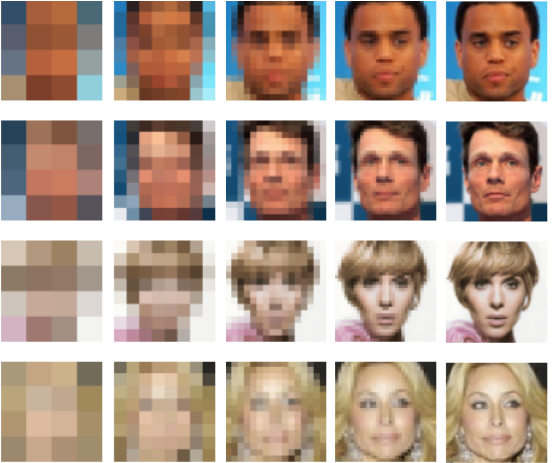
\includegraphics[width=0.7\textwidth]{images/ground_truth/gt_resolutions.png}
\caption{Slike iz skupa CelebA rastuće rezolucije, od $4 \times 4$ do $64 \times 64$.}
\label{gt_resolutions}
\end{figure}

Prilikom generiranja slika za demonstraciju, koristimo se "trikom odsijecanja" \engl{truncation trick}: uzorkujemo iz normalne razdiobe, ali ako prelazi određeni prag, uzorak odbacujemo i ponavljamo postupak. Ideja je da ovim pristupom poboljšavamo kvalitetu generiranih slika, ali gubimo na određenom stupnju raznolikosti. Napomenimo još da se prilikom evaluacije rezultata ovime ipak ne koristimo.

Uzorak slika iz odabranog modela nakon treniranja uz veličinu minigrupe od 16 primjera te podešavanje parametara prikazani su na slici \ref{generated_16bs_fine_tune}.

\begin{figure}[h]
\centering
		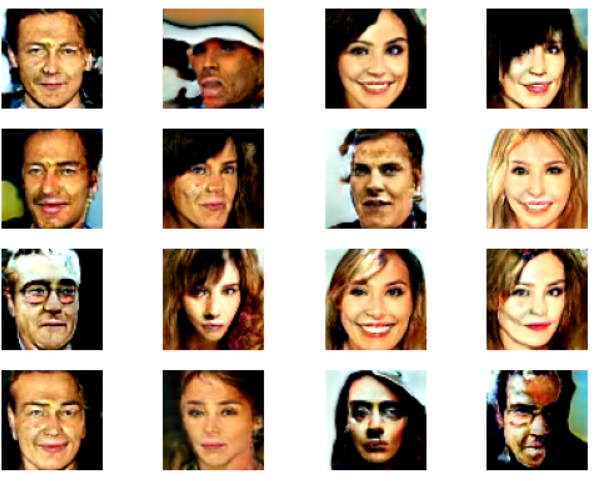
\includegraphics[width=0.8\textwidth]{images/generated/16bs_best_fid.png}
\caption{Uzorak slika generiran odabranim modelom uz minigrupu od 16 primjera}
\label{generated_16bs_fine_tune}
\end{figure}

FID određen na skupu za testiranje (oko 50000 slika) kroz epohe na najvišoj rezoluciji prikazan je u tablici \ref{tablica_fid_16bs}. Iako ne postoji konsenzus pomoću kojeg skupa odrediti FID, prema \todo{are all gans created equal} odlučili smo se za skup za testiranje radi pravednije procjene.

\begin{table}[h]
\caption{FID vrijednosti modela kroz epohe treniranja}
\begin{center}
\begin{tabular}{ |c|c|c|c|c|c|c|c|c|} 
 \hline
 Epoha & 1 & 2 & 3 & 4 & 5 & 6 & 7 & 8 \\
 \hline
 FID & 2221.56 & 2563.519 & 2042.023 & 2973.36 & 2061.18 & 2025.02 & 2222.09 & 1770.68 \\
 \hline
\end{tabular}
\end{center}
\label{tablica_fid_16bs}
\end{table}

Da bismo dodatno podesili parametre, trebali smo odabrati epohu da inicijaliziramo parametre temeljem te vrijednosti. Odabrali smo treću epohu, iako imamo i slučajeve gdje je FID vrijednost niža. Ovo se temelji na pregledavanju slika koje je model generirao u pojedinom stadiju. Primjer generiranih slika u zadnjoj epohi treniranja prikazan je na slici \ref{generated_lowest_fid}.

\begin{figure}[h]
\centering
		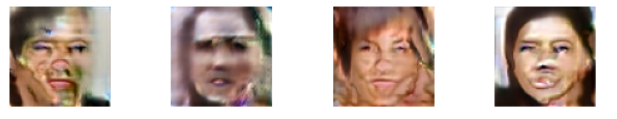
\includegraphics[width=0.8\textwidth]{images/generated/16bs_lowest_fid.png}
\caption{Uzorak slika generiran modelom s najmanjim FID-om}
\label{generated_lowest_fid}
\end{figure}

Osim ovog pristupa, pokušan je i pristup gdje povećamo veličinu grupe na 64 primjera, a težine modela nižih rezolucija s najboljim FID-om koristimo kao osnovu za više rezolucije. Međutim, nisu dobivena značajna vizualna poboljšanja. 

U kasnijim epohama treniranja, vrlo lako se mogla primijetiti pojava \textit{mode collapse}. Slika \ref{mode_collapse} pokazuje kako to točno izgleda. 

\begin{figure}[h]
\centering
		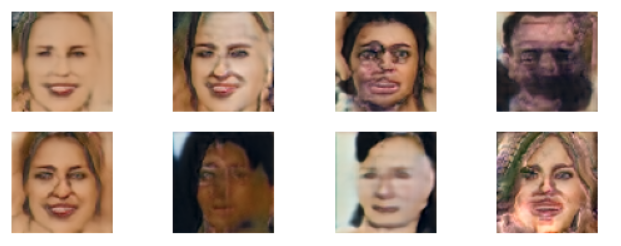
\includegraphics[width=0.8\textwidth]{images/generated/mode_collapse.png}
\caption{Primjer pojave \textit{mode collapse}}
\label{mode_collapse}
\end{figure}

Jedno zanimljivo svojstvo koje posjeduju generativne suparničke mreže jest da se aritmetika nad latentnim vektorima $\vec{z}$ na neki način preslikava u semantiku na generiranim slikama. Slika \ref{interpolation} prikazuje slike generirane latentnim vektorima dobivenim interpolacijom između dva početna latentna vektora. 

\begin{figure}[h]
\centering
		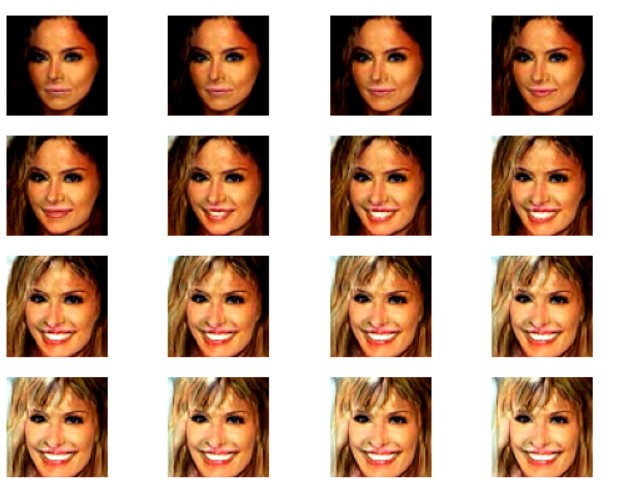
\includegraphics[width=0.8\textwidth]{images/generated/interpolation_1.png}
\caption{Slike dobivene interpolacijom}
\label{interpolation}
\end{figure}

Možemo primijetiti da se između početne i završne slike događa postupna promjena u izrazu lica, boji kose i tenu. To upućuje na zaključak da je model ulazni vektor uspio upotrijebiti kao uputu za generiranje semantičkih elemenata lica, iako raspolaže samo s pojedinim pikselima - u stanju je steći znanje o strukturi lica. Ovu pojavu nazivamo raspetljanošću \engl{disentaglement} latentnog prostora i opisuje sposobnost modela da različita povezana područja ulaznog prostora namijeni za generiranje pojedinih elemenata slike, ali tako da su ta područja specijalizirana. Iako trenutno imamo vrlo malo kontrole nad izlazom modela, raspetljanost ulaznog prostora mogla bi se u budućnosti iskoristiti da riješimo i taj izazov.
\chapter{Zaključak}
U ovom smo radu predstavili koncept generativnih suparničkih mreža u kontekstu generiranja slika. Između ostalog, pozabavili smo se njihovom osnovnom idejom, teorijskom podlogom te predstavili elemente od kojih se sastoje, zajedno s pregledom relevantnih radova. Napokon, prikazali smo primjenu koncepta na skupu slika koji se uobičajeno koristi u praksi te razjasnili odluke koje smo morali donijeti pri implementaciji.

Iz svega navedenoga, možemo zaključiti da su generativne suparničke mreže izrazito moćan model s vrlo dobrim rezultatima u generiranju slika. Međutim, brojna pitanja u ovom području su još uvijek neodgovorena.

Jedan od najvažnijih problema jest nestabilnost njihova treniranja, odnosno visoka osjetljivost na promjenu hiperparametara, kao i reproducibilnost rezultata. Osim toga, važan je izazov i mogućnost kontrole pri generiranju slika. Iako određeni napretci u tom području postoje, ideja ugradnje pretpostavki u generiranje slika je tek u svom početnom stadiju. I za kraj, neadekvatno odgovoreno pitanje je i problem evaluacije generiranih slika, odnosno prevencija prenaučenosti. 

Bilo kako bilo, možemo očekivati da će, uz stvaranje sve boljih i boljih skupova podataka kao i porast računalne moći, i ovi izazovi  biti razriješeni. 

\bibliography{literatura}
\bibliographystyle{fer}

\begin{sazetak}
Generativne suparničke mreže moćna su klasa dubokih modela i vrlo aktivno područje istraživanja. U ovom radu predstavljamo njihov osnovni koncept te iznosimo ideju iza generativnih modela općenito. Budući da se model u najširem smislu temelji na suradnji između dvije duboke neuronske mreže, na visokoj razini pojašnjavamo kako i one funkcioniraju. Iznosimo i uobičajeno korištene osnovne slojeve neuronskih mreža korištenih mreža te pregled dosadašnjeg rada. I za kraj, pokazujemo implementaciju generativnih suparničkih mreža temeljenih na progresivnom rastu i njihovu primjenu pri generiranju slika ljudskih lica koristeći skup podataka CelebA rezolucije $64 \times 64$ te vrednujemo rezultate.

\kljucnerijeci{generativne suparničke mreže, duboko učenje, generiranje slika, generativni model, progresivni rast mreža}
\end{sazetak}

% TODO: Navedite naslov na engleskom jeziku.
\engtitle{Application of Generative Adversarial Networks on Image Generation}
\begin{abstract}
Generative adversarial networks are a powerful class of deep learning models and a particularly active field of research. In this work, we present the basic idea of generative models and the concept of generative adversarial networks. Since this model is, in the broadest sense, based on the cooperation of two neural networks, we present a broad overview of this concept as well. We note the neural layers usually used in such a system and the work done so far. Finally, we implement a variant of this concept based on progressive growing and apply it to generation of images of human faces of $64 \times 64$ resolution  using the CelebA dataset and evaluate our results.

\keywords{generative adversarial networks, deep learning, image generation, generative models, progressive growing}
\end{abstract}

\end{document}
